\chapter{In-medium transport model for hard partons}
\cite{ATLAS-Collaboration:2012iwa,Abelevetal:2014dna,STAR:upgrade-hf,Adare:2015kwa,CMS:2017dec}
\cite{Wang:1994fx,Zakharov:1996fv,Baier:1996sk,Zakharov:1997uu,Arnold:2002zm,Gyulassy:2003mc,Kovner:2003zj,Jeon:2003gi,CasalderreySolana:2007pr,Djordjevic:2008iz,Bass:2008rv,Schenke:2009gb,Majumder:2009zu,Majumder:2010qh,Armesto:2011ht,Zapp:2011ya,Ovanesyan:2011xy,Kang:2014xsa,Cao:2016gvr,Kauder:2018cdt,Cao:2017zih}.

Hard partons are predominately created in perturbative scatterings in the earliest stage of relativistic heavy-ion collision.
The distribution of the hard partons gets modified by its in-medium propagation and therefore whose final states carries information about the medium properties, as well as hard-soft interactions that are interested.

Among the many ways of describing the in-medium evolution of hard partons, 
transport approach has its unique advantage. 
Here, by transport approach, we are referring to a general class of transport model that does the time evolution of a semi-classical particle distribution function.
Transport models can be often formulated as simulation on the particle level, which provides easy coupling to local properties of a dynamically evolving and fluctuating medium, with exclusive information of the final states.

There are also challenges associated to the transport modeling in high energy collision.
First, there are different assumptions of the interactions between the hard parton and soft medium.
Two commonly assumed extremes are:
\begin{itemize}
\item[1] A weakly coupled picture: medium are consists of perturbative quasi-particles (scattering centers) whose distribution is close to local thermal equilibrium.
Hard partons scatters pertrubtively with these well separated scattering centers. The dynamics are described by a Boltzmann equation.
\item[2] Diffusion picture: interactions between the medium and the hard parton are frequent and soft, many body effects and non-perturbative effects can be important. The statistical effect of these interactions are modeled by a drag and a diffusion coefficient. The dynamics are solved using a Langevin equation.
\end{itemize}
These two commonly used approaches are not necessarily mutually exclusive, and can have different range of application. 
For example, the effect of a large part of soft momentum exchange processes in the perturbative calculation can be well modeled by a diffusion equation.
These drastically different assumptions on the interaction between the medium and the hard probe is largely due to our inadequate theoretical tools in describing the QGP medium in the strongly coupled regime.
On the one hand, this becomes the model uncertain intrinsic to transport approach, until one founds convincing way of interpreting the strongly coupled QGP medium from first principal.
On the other hand, this also becomes a chance to extract the properties of the medium through a systematic model-to-data comparison. 
An ultimate goal would be answering whether quasi-particle degrees of freedom is an effective description of sQGP using hard probes.

A second difficult associated to the semi-classical transport modeling is the treatment of quantum coherence effect.
Indeed, a quantum transition will always be bounded by the uncertainty principal: a process with momentum scale $Q$ can not be localized within a space (time) extend of $1/Q$.
While in the semi-classical transport model, one always specify a local point in space-time where the interaction takes place.
This is of course validate if the momentum scale $Q$ is high enough that $1/Q$ is much smaller than the resolution that the transport model concerns, e.g., characterized by the mean-free-path in Boltzmann equation.
However, soft and collinear divergence of QCD bremsstrahlung (or more generally, parton branching) processes generates an abundance of small-$Q$ events whose spatial extents can be much greater than the na\"ive expectation of mean-free-path. 
This happens for certain phase space of the vacuum parton shower as well as the medium-induced parton shower.
The vacuum parton shower are often solved as a vitality evolution with the  time variable integrated out, while the transport equation is an evolution in time with virtuality integrated out, we shall postpone the discussion to the next section.
This section focus on the medium induced part, where the QCD in-medium branching receives contribution from multiple scattering centers that leads to the QCD analog of the Landau-Pomeranchuk-Migdal (LPM) effect, and the radiation pattern is changed qualitatively.
When this happens, strictly speaking, the semi-classical transport equation is not the appropriate tool for these processes.
However, considering the advantages of the transport formulation, we would like to develop a minimum set of modification to the semi-classical transport that can mimic some quantum effect of in-medium parton branching.


As an overview of the section and our goals in developing the transport model,
We start with introduction of widely used transport equations: the (linearized ) Boltzmann equation and the Langevin equation.
Considering the elastic interaction first, we try to combine these two transport approach into a hybrid one by introducing a cut-off distinguishing hard and soft momentum transfer process.
After that, we introduce the theory related to QCD in-medium parton branching processes and discuss its various approximations and also the exact solutions.
With these theoretical insights, we developed a ``modified Boltzmann transport" approach in treating the in-medium parton branching approximately.
Finally, we compare the simulated results the transport model to the theoretical expectations to validate the implementation in different regime.
We will show that the modified transport approach can reasonable describes the longitudinal structure of the medium-induced splitting vertex for different channels $q\rightarrow q+g$, $g\rightarrow g+g$ and $g\rightarrow q+\bar{q}$.
Treatment of the heavy quark masses effect, and running coupling is investigated at the very end.

\cite{PhysRev.103.1811,Wang:1994fx,Zakharov:1996fv,Zakharov:1997uu,Baier:1996kr,Baier:1996sk}

\cite{Cao:2013ita,ColemanSmith:2012vr,Xu:2004mz,Zapp:2011ya,Gossiaux:2012cv,Park:thesis}.

\cite{Arnold:2002zm,Arnold:2008zu,Arnold:2009mr,Baier:1996kr,Baier:1998yf}. 

\section{The Boltzmann equation}
The Boltzmann equation evolves the transport of particles' distribution function under the effect of localized collision. 
By localization, it means that the time scale of the collision has to be much smaller compared to the mean free-path $\tau \ll \lambda$. 
Therefore, the collision probability can be evaluated using local particle distribution function.
Also the calculation of the few body collision processes is not significantly affected by the presence of the other particles, because the probability to interact with another particle during this collision is small, $P \approx \tau/\lambda \ll 1$.
At weak coupling, we will see in the next section that this is indeed the case for elastic collision, and soft and large radiation, but not high energy radiation where $\tau$ is actually much greater than the mean-free-path, and hence ``non-local".
Accordingly, the Boltzmann formulation and solvers needed to be modified to take into this non-local effect.
We postpone the related discussion later and shall assume in this subsection that the interactions are local. 

Considering two-body to two-body (elastic) and two-body to three-body (inelastic, including the reverse process) processes take the Boltzmann equation for particle specie $a$ takes the following form,
\begin{eqnarray}
\frac{\partial f^a}{\partial t} + \vec{v}\cdot\frac{\partial f^a}{\partial \vec{x}} + \frac{\partial E}{\partial \vec{x}}\cdot\frac{\partial f^{a}}{\partial \vec{p}} = - \sum_{b,c,d}\mathcal{C}_a^{a+b\leftrightarrow c+d}- \sum_{b,c,d,e}\mathcal{C}_a^{a+b\leftrightarrow c+d+e}
\end{eqnarray}
On the left hand side, the distribution function $f^{a}(t, \vec{x}, p)$ undergoes transport with velocity $\vec{v} = \partial E/\partial \vec{p}$, and a possible potential potential force $\vec{f} = -\partial E/\partial \vec{x}$.
On the right hand side of the equation, the $2\leftrightarrow 2$ and $2\leftrightarrow 3$ collision term are functions of the distribution functions, changing the distribution function through a gain term and a loss term in the one particle phase-space.
The summation of over $b,c,d,e$ iterates over all other particle species including $a$.
Using the elastic process as an example and neglecting degeneracy of the internal quantum number for simplicity, the collision term for a specific process is,
\begin{eqnarray}
\mathcal{C} &=& \mathcal{C}_\textrm{loss} + \mathcal{C}_\textrm{gain}\\
&=& \int f^a(p_1)f^b(p_2)[1+\epsilon^c f^c(p_3)][1+\epsilon^d f^d(p_4)] \overline{|M|^2}(p_1^a, p_2^b; p_3^c, p_4^d) d[PS]_{bcd} \\\nonumber
&-& \int f^c(p_3)f^d(p_4)[1+\epsilon^a f^a(p_1)][1+\epsilon^b f^b(p_2)] \overline{|M|^2}(p_3^c, p_4^d; p_1^a, p_2^b) d[PS]_{bcd} \\
&=& \int \left\{
f^a(p_1)f^b(p_2)[1+\epsilon^c f^c(p_3)][1+\epsilon^d f^d(p_4)] \right. \label{eq:collision-term:symmetry} \\\nonumber
&& \left.- f^c(p_3)f^d(p_4)[1+\epsilon^a f^a(p_1)][1+\epsilon^b f^b(p_2)]\right\}
\overline{|M|^2} d[PS]_{bcd} 
\end{eqnarray}
Where the crossing symmetry of the matrix-elements has been used in the last line of the equation ($\overline{|M|^2}(p_1^a, p_2^b; p_3^c, p_4^d) = \overline{|M|^2}(p_3^c, p_4^d; p_1^a, p_2^b) = \overline{|M|^2}$), and the phase-space integral is 
\begin{eqnarray}
d[\textrm{PS}]_{bcd} = \prod_{i\in {b,c,d}}\frac{dp_i^3}{2E_i (2\pi)^3} (2\pi)^4 \delta^{4}(p^a_1+p^b_2 - p^c_3-p^d_4).
\end{eqnarray}
The $epsilon = 0, -1, 1$ corresponds to classical, Fermi-Dirac, and Bose-Einstein statistics depending on the nature of the particle.

The first term in the integration represents the loss of type-$a$ particle in the phase-space around point $(x, p_1)$ due to elastic collisions, and the second term represents the gaining of type-$a$ due to the reverse processes.
The symmetry in the microscopic matrix-element is very important for the kinetic equation and ensure the detailed balance: the probability to transition from one microscopic state to anther equals its reverse process.
The detailed balance is also important for the reach of thermalization of the system. 
Assume the system has been evolved in a cell with fixed volume and there is no spatial variance of the distribution function.
Then using the form of the collision term in Eq. \ref{eq:collision-term:symmetry}, one can see that the static solution of the distribution function has to satisfy the relation,
\begin{eqnarray}
f^a f^b (1+\epsilon f^c) (1+\epsilon f^d) = f^c f^d (1+\epsilon f^a) (1+\epsilon f^b),
\end{eqnarray}
for the entire phase-space and every combination of particle species.
Therefore, the following combination is conserved for each reaction channel.
 \begin{eqnarray}
\frac{f^a}{(1+\epsilon^a f^a)} \frac{f^b}{(1+\epsilon^b f^b)}
= \frac{f^c}{(1+\epsilon^c f^c)} \frac{f^d}{(1+\epsilon^d f^d)}
\end{eqnarray}
The nature conservation one expect is the energy-momentum conservation, and therefore one solution to the previous equation is,
\begin{eqnarray}
\frac{f^a}{(1+\epsilon^a f^a)} = e^{-\beta \mu_a-\beta p\cdot u}
\end{eqnarray}
for every particle species with parameters $\mu, \beta$ and a four vector $u$ ($u^2 = 1$). 
So the static solution of the distribution is 
\begin{eqnarray}
f^a(p) = \frac{1}{ e^{\beta \mu_a+\beta p\cdot u} - \epsilon^a} \label{eq:thermal}\\
\mu_a +\mu_b = \mu_c + \mu_d \label{eq:chem}
\end{eqnarray}
The fist line is the thermal distribution as expected that characterizes the kinetic equilibrium of the system, and the second line is the requirement for reaching chemical equilibrium. 
And one can identify the $\beta$ and $\mu$ parameter as the inverse temperature and chemical potential. The $u$ vector is the flow velocity of the cell as can be seen from the average velocity,
\begin{eqnarray}
\left\langle \frac{p^\mu}{M} \right\rangle = \frac{\int f(p) \frac{p^\mu}{M} dp^3}{\int f(p) dp^3} = \frac{\int f(p) \frac{p^\mu}{M} dp^3}{\int f(p) dp^3} = u^\mu
\end{eqnarray}

\section{Linearization of the Boltzmann equation and the diffusion limit}
The full Boltzmann equation is a coupled differential-integral equation for all distribution function and has non-linearities. 
As a result, the analytic solutions for even simple form of interaction is almost impossible.
The numerical solution / simulation is also a highly non-trivial task.
However, under certain circumstances, a linearization of the Boltzmann equation is possible and greatly simplifies both analytic analysis as well as the numerical simulation.

The hard particles (jet partons, heavy flavors) are initial produced in perturbative processes with a large $p_T$ or a large mass $M \gg T$. 
The perturbative production cross-section drops fast with the increase of $p_T$ and $m_T$, so hard partons are very rare in actually event. 
Therefore the occupation number of hard parton is a small number $f_H \ll 1$.
One can neglect the quantum statistics terms in the Boltzmann equation for them $1+\epsilon f_H \approx 1$.
For the Boltzmann equation of hard partons, the collision terms with more than one uncorrelated hard particles in the initial state can also be neglected since these contributions is proportional to $f_H^2 \ll f_H$. 
Finally, we also assume that the response of the bulk of the particles to the hard particles is small, and shall neglect any collision terms that involve a hard parton in the Boltzmann equation for the bulk distribution function.
Under these approximations, one arrived at a set of equations that is linearized with respect to the hard partons:
\begin{eqnarray}
\frac{df_H}{dt} &=& -\mathcal{C}_H[f_H, f_{\textrm{bulk}}] \label{eq:hard-bulk-eq}\\
\frac{df_{\textrm{bulk}}}{dt} &=& -\mathcal{C}[f_{\textrm{bulk}}]
\end{eqnarray}
Here the collision term $\mathcal{C}_H$ is linear with respect to $f_H$.

For the bulk particles, one still have a complex set of coupled equation to solve. 
However, a great simplification can be made by observing that the time it takes for the bulk particles to reach local thermalization is much shorter than the hard particles relaxation time, so a zeroth order approximation would be using the local thermal distribution of Eq. \ref{eq:thermal}.
The space-time evolution of the temperature $T$, chemical potential $\mu$ and flow velocity $u$ can be obtained from a hydrodynamic solution that also assumes a close-to-local thermalization of the bulk medium.
Replacing the bulk medium distribution function by the thermal in Eq. \ref{eq:hard-bulk-eq}, one arrives at a closed (linearized) equation for the hard particles.
Here we write down the equation assuming both the classical statistics and the conservation of the hard parton's species, and only elastic collision term is shown for simplicity,
\begin{eqnarray}
\frac{\partial f^H}{\partial t} + \vec{v}\cdot\frac{\partial f^H}{\partial \vec{x}} &=& -\sum_{b} \int \left\{
f^H(p_1)f^b_{eq}(p_2) - f^H(p_3)f^b_{eq}(p_4)\right\}
\overline{|M|^2} d[\textrm{PS}]_{234} \\
&=& - \int \left\{
f^H(p_1) w(p_1; p_3) - f^H(p_3) w(p_3, p_1)\right\}\frac{dp_3^3}{2E_3 (2\pi)^3}
\end{eqnarray}
Where the $w(p; p')$ are the transition probability density for a particle with momentum $p$ into momentum state $p'$,
\begin{eqnarray}
w(p; p') = \sum_b\int f_{eq}^b(p_2) \overline{|M|^2}(p, p_2; p', p_4) d[\textrm{PS}]_{24}
\end{eqnarray}

This seems to be a great simplification to the original coupled equation. However, the use of locally equilibrium of the bulk particle distribution function is a strong assumption. 
The degree of local thermalization in realistic events is still an open question, especially at early stages. 
Even if the system is close to local thermal equilibrium, whether it can be understood in terms of the quasi-particle degrees of freedom that has been described using semi-classical distribution function is a different question.
In an extreme weakly coupled system $g\ll 1$, one expected the local pressure and energy density can be explained in terms of the fundamental degrees of freedom: quarks and gluons, with perturbative corrections.
But with a large $g$ estimated from phenomenology studies, such a perturbative description may not be most efficient way of understanding the bulk medium and non-perturbative physics can play an essential row. 
This interpretation of the medium in terms of microscopic degree-of-freedom seem to be a an unavoidable problem of the Boltzmann equations, however, it is possible to ``integrate out" the microscopic details of the medium if the interaction in the soft limit of interaction.
In the soft momentum transfer $q = p'-p$ limit  $|q| \ll |p|$, the change in distribution function can be expanded to the second terms in the $q$, and the linearized Boltzmann equation reduces to the Fokker-Planck type of equation,
\begin{eqnarray}
\frac{\partial f}{\partial t} + \vec{v}\cdot\frac{\partial f}{\partial \vec{x}} &=& - \int \left\{
f(p) - \left[f(p) +  \vec{q}\frac{\partial f}{\partial\vec{p}} + \frac{1}{2}\vec{q}\vec{q}\frac{\partial^2 f}{\partial\vec{p} \partial\vec{p}} \right]
\right\} w(p',p)\frac{dp_3^3}{2E_3 (2\pi)^3} \\
&=& - \int \left\{ \vec{q}\frac{\partial f}{\partial\vec{p}} - \frac{1}{2}\vec{q}\vec{q}\frac{\partial^2 f}{\partial\vec{p} \partial\vec{p}}
\right\} w(p',p)\frac{dp_3^3}{2E_3 (2\pi)^3} \\
&=&  -A(p) \frac{\partial f}{\partial\vec{p}} + \frac{1}{2}B(p)\frac{\partial^2 f}{\partial\vec{p} \partial\vec{p}}
\end{eqnarray}
The transport coefficient are defined as
\begin{eqnarray}
A(p) &=& \int w(p,p+q) q \frac{dp_3^3}{2E_3 (2\pi)^3}\\
B(p) &=& \int w(p,p+q) q q \frac{dp_3^3}{2E_3 (2\pi)^3}
\end{eqnarray}
which are the first and second moments of the transition probability.
One remark is that although the form of the Fokker-Planck equation can be derived as the diffusion (soft) limit of the linearized version of the Boltzmann equation, its range of applicability can be different.
This is because the transport coefficient is well defined in general regardless of whether one assumes quasi-particle type microscopic dynamics.
In fact, in our final model, we replace the soft sector of the Boltzmann equation with the Fokker-Planck equation so that the use of ``medium quasi-particles" are restricted to hard momentum transfer processes.
Moments beyond second order is dropped in deriving the Fokker-Planck equation, this is justified if the interaction is frequent enough so that within the smallest time scale that is concerned, there is already many interactions such that a statistical description of the effect of interaction is adequate in terms of the first (mean) and the second moments (standard deviation).
However, if the physical processes is rare within the considered time scale, when fluctuation characterized by higher moments of the transition probability is very important and a diffusion approximation will not be a good proxy in describing its effect.
For this reason, we will later show that the diffusion approximation  does not work for radiation with a large gluon energy $\omega \gg T$.

\section{The elastic process in the medium}
Elastic collision are usually refers to the processes where the number of hard partons are conserved.
In a quasi-particle picture of the QGP, the hard parton can collide with medium partons and transfer a certain amount of energy to the medium.
These processes can be calculated at leading order in the weakly coupled theory, where the collision cross-section is calculated using the dressed gluon propagator inside the medium,
\begin{eqnarray}
D^{\mu\nu}(\omega, k) = \frac{\delta^{\mu 0}\delta^{\nu 0}}{k^2 - \Pi_L(\omega, k)} + \frac{\hat{P}_T^{\mu\nu}}{\omega^2 - k^2 - \Pi_T(\omega, k)}
\end{eqnarray}
Due to the presence of the medium, the dressed propagator lost its Lorentz invariance and depends on complicated in-medium self energy $\Pi_T$ and $\Pi_L$.
And the resulting cross-section formula will be equally complicated.
Fortunately, it has been shown recently in [] that a simplification is possible at leading order in rewriting the elastic processes as large-angle scattering and small-angle diffusion.
In such an approach, a cut-off in momentum transfer $Q_\textrm{cut}$ is introduced, with the range formally satisfying $gT \ll Q_\textrm{cut} \ll T$.
For processes with momentum transfer to the medium larger than the cut-off  (hard-mode) the medium screening effect is neglected and vacuum matrix-element is used as a proxy.
While for processes smaller than the cut-off (soft-mode), the propagator receives significant contribution from the screen effect.
The soft processes happens frequent and only involves small momentum transfer; therefore, its statistical effect over a finite amount of time can be efficiently captured by the diffusion dynamics.
The resultant transverse and longitudinal diffusion constant has been calculated by [] to be,
\begin{eqnarray}
\hat{q}_L = g^2 C_R T m_\infty^2  \ln\left(1+\frac{Q_{\textrm{cut}}^2}{m_\infty^2}\right) \\
\hat{q} = g^2 C_R T m_D^2  \ln\left(1+\frac{Q_{\textrm{cut}}^2}{m_D^2}\right).
\end{eqnarray}
$m_\infty^2 = m_D^2/2$ is the asymptotic gluon thermal mass.

This separation allows the following modeling of the elastic interaction between hard parton and the medium,
\begin{eqnarray}
\frac{df}{dt} = \mathcal{D}[f] + \mathcal{C}^{2\leftrightarrow 2}[f].
\end{eqnarray}
So that the particle is continuously evolved by the diffusion process while undergoing occasionally large-angle scatterings.
Of course, we would like to verify that this separate cut-off dependence in the diffusion and scattering component indeed cancels for physical observations at sufficiently small coupling.

The theoretical assumption of a quasi-particle QGP and using leading order resummed propagator really replies on the weakness of the coupling constant $g$. 
While the phenomenological value of $g$ is in fact not small, and one may question whether the interaction between the hard parton and the medium receives a significant non-perturbative contribution.
Although the non-pertubative physics varies in different calculations, their dynamical effect are often modeled by a diffusion processes.

\section{Transport approach in the incoherent limit}
In this section, we describe the Monte Carlo model in detail. The partonic processes are categorized into elastic (particle number conserving) and inelastic processes (particle number non-conserving). 
The inelastic processes are further divided into parton-splitting and parton-jointing contribution. 
In this section, we shall first proceed using local and incoherent calculation of such processes and will discuss in great detail in the next section on including the LPM effect in a Boltzmann-like transport approach.

The elastic interaction between hard parton and medium is separate into a large-momentum transfer (hard) and a small-momentum transfer (soft) part.
The switching scale is chosen to be proportional to the Debye mass square $Q_{\textrm{cut}}^2 = c m_D^2$, where $c$ is a parameter.
Respectively, the inelastic processes are also separated into diffusion-induced slitting / jointing processes, and large-$Q$ matrix-element based inelastic scattering contribution.

The large-$Q$ collisions are solved by a linearized Boltzmann equation with using collision rates calculated with vacuum matrix-elements, while the soft interactions are approximated by a diffusion process and is solved by Langevin equations.
This combined Langevin and linearized Boltzmann dyanmics is solved on the particle level using a two step approach,
\begin{eqnarray}
\vec{x}(t+\Delta t) &=& \frac{\vec{p}}{E}\Delta t\\
\vec{p}_{\textrm{int}} &=& \vec{p} - \eta_D \vec{p} \Delta t + \vec{\xi}(t) \Delta t\\
\Delta t\frac{dR(T, \vec{v}, \vec{p}_{\textrm{int}})}{d\vec{p}^3} &\xrightarrow{\textrm{sampling}}& \vec{p}(t+\Delta t)
\end{eqnarray}
Where the particle first does free transport, and then its momentum be updated with diffusion dynamics to get an intermediate $\vec{p}_{\textrm{int}}$. 
Then, the particle under goes collision according to the reaction probability within $\Delta t$, and the final states are obtained by sampling the differential collision rate.
The diffusion dynamics consists of a thermal random force such that,
\begin{eqnarray}
\left\langle\xi_i(t)\xi_j(0)\right\rangle = \delta(t) \left(
\frac{p_i p_j}{p^2}\hat{q}_{S, L} + \left(
\delta_{ij}-\frac{p_i p_j}{p^2}
\right)\frac{\hat{q}_S}{2} 
\right)
\end{eqnarray}
Because we require that the diffusion dynamics only accounts for soft momentum transfer processes, its transport coefficient is obtained by integrating the leading order collision kernel upto the momentum $Q_{\textrm{cut}}$,
\begin{eqnarray}
\hat{q}_S = \int dq^2 \frac{\alpha_s m_D^2 T}{q^2 (q^2+m_D^2)} 
\label{eq:qS} \\
\hat{q}_{S,L} = \int dq^2 \frac{\alpha_s m_\infty^2 T}{q^2 (q^2+m_\infty^2)}
\label{eq:qSL} 
\end{eqnarray}
with the drag coefficient determined by the Einstein relation,
\begin{eqnarray}
\eta_D = \frac{\hat{q}_{S,L}}{2ET} - \frac{d\hat{q}_{S,L}}{dp^2} - \frac{2\hat{q}_{S,L} - 2\hat{q}_S}{2p^2}
\end{eqnarray}
For the large-$Q$ scattering processes, the collision rates for the $2\rightarrow 2$ and $2\rightarrow 3$ scatterings are obtained by integrating the vacuum matrix-element,
\begin{eqnarray}
R = \frac{d}{2E_1}\int  \frac{d^3p_2}{2E_2(2\pi)^3} f_0(p_2)2\hat{s} \int_{-\hat{s}}^{Q_{\textrm{cut}^2}}\frac{d\sigma}{d\hat{t}}d\hat{t}
\end{eqnarray}
The integration is restricted to large momentum transfer above $Q_{\textrm{cut}}$ and therefore we do not impose additional screening effect to regulate the matrix-element.
For the incoherent diffusion-induced splitting rate, we borrow the expression from \cite{Cao:2017hhk} stripping the time-dependent phase factor,
\begin{eqnarray}
R = \int d k_\perp^2 dx \frac{\alpha_s P(x) \hat{q}^S}{2\pi (k_\perp^2 + m_\infty^2)^2}
\end{eqnarray}
where a gluon thermal mass is added to screen the divergence.
For the reverse processes $3\rightarrow 2$  and $2\rightarrow 1$ processes, similar reaction rate can be written down.

The vacuum matrix-element is used for the large-$Q$ elastic and inelastic scatterings.
In this work, the $2\rightarrow 2$ matrix-element only includes the $\hat{t}$-channel contribution.
Regarding the $2\rightarrow 3$ matrix-element, in previous study \cite{Ke:2018tsh}, we used to employ an improved version of the original Gunion-Bertsch cross-section that works under the limits $k_\perp, q_\perp \ll \sqrt{s}$ and $x q_\perp \ll k_\perp$ \cite{PhysRevD.25.746,Fochler:2013epa,Uphoff:2014hza}.
In the present study, we keep improving the matrix-elements by following the derivation in \cite{Fochler:2013epa} while relaxing the condition $x q_\perp \ll k_\perp$.
Therefore the updated matrix-elements contain the correct vacuum splitting function in the collinear limit.
We summarize the matrix-elements here and have attached a derivation in the appendix,
\begin{eqnarray}
\overline{|M^2|}_{g+i\rightarrow g+g+i} &=& \overline{|M^2|}_{g+i\rightarrow g+i} P_{gg}^{g(0)}  D_{gg}^{g}\\
\overline{|M^2|}_{g+i\rightarrow q+\bar{q}+i} &=& \frac{C_F d_F}{C_A d_A}\overline{|M^2|}_{g+i\rightarrow g+i} P_{q\bar{q}}^{g(0)} D_{q\bar{q}}^{g}\\
\overline{|M^2|}_{q+i\rightarrow q+g+i} &=& \overline{|M^2|}_{q+i\rightarrow q+i} P_{qg}^{q(0)} D_{qg}^{q},
\end{eqnarray}
where $P_{bc}^{a(0)}(x)$ are vacuum splitting functions from parton $a$ to partons $b$ and $c$. Index $i$ represent a quark / anti-quark or a gluon.
The two body matrix-elements that enters the $2\rightarrow 3$ matrix-element is always required to be the $t$-channel contribution.
\begin{eqnarray}
P_{gg}^{g(0)}  &=& g^2  C_A\frac{1+x^4+(1-x)^4}{x(1-x)}\\
P_{qg}^{q(0)} &=& g^2  C_F\frac{1+(1-x)^4}{x}\\
P_{q\bar{q}}^{g(0)} &=& g^2  \frac{N_f}{2}\left(x^2+(1-x)^4\right)
\end{eqnarray}
The $D_{bc}^{a}$ contains the interference structure,
\begin{eqnarray}
D_{qq}^{g} &=& 
C_A(\vec{a}-\vec{b})^2 + C_A(\vec{a}-\vec{b})^2 \\\nonumber
&-& C_A (\vec{a}-\vec{b})\cdot (\vec{a}-\vec{c})
\\
D_{q\bar{q}}^{g} &=& 
C_F(\vec{a}-\vec{b})^2 + C_F(\vec{a}-\vec{b})^2 \\\nonumber
&-& (2C_F-C_A) (\vec{a}-\vec{b})\cdot (\vec{a}-\vec{b})
\\
D_{qg}^{q} &=& 
C_F(\vec{c}-\vec{a})^2 + C_F(\vec{c}-\vec{b})^2 \\\nonumber
&-& (2C_F-C_A) (\vec{c}-\vec{a})\cdot (\vec{c}-\vec{b})
\end{eqnarray}
with the vectors given by
\begin{eqnarray}
\vec{a} = \frac{\vec{k}_\perp - x\vec{q}_\perp}{(\vec{k}_\perp - x\vec{q}_\perp)^2};
\vec{b} = \frac{\vec{k}_\perp - \vec{q}_\perp}{(\vec{k}_\perp - \vec{q}_\perp)^2};
\vec{c} =  \frac{\vec{k}_\perp}{\vec{k}_\perp^2}.
\end{eqnarray}


Combining all these processes, we summarize our linearized-Boltzmann plus Langevin equation into,
\begin{eqnarray}
\frac{df}{dt} = \mathcal{D}[f] + \mathcal{C}_{1\leftrightarrow 2}[f] + \mathcal{C}_{2\leftrightarrow 2}[f] + \mathcal{C}_{2\leftrightarrow 3}[f].
\end{eqnarray}
The distribution function of the hard parton under goes soft diffusion and diffusion induced-radiation. 
Hard collision with the medium are included as $2\leftrightarrow 2$ and $2\leftrightarrow 3$ collision terms.
The next section devotes to the inclusion of LPM effect to such an incoherent transport equation.

\section{Monte Carlo solver of the linearized Boltzmann equation}
This subsection discuss the technical of solving the linearized Boltzmann equation using particle-based simulation.
This method starts from representing the distribution function by particle states. 
For linearized Boltzmann equation, it is sufficient to consider the dynamics of one such particle.
The particle undergoes free-transport in between subsequent collisions, and differential collision probability per unit time, the collision rate, is simply the collision integral, with the distribution function replaced by a delta-distribution $\delta^{3}(x-x'- v(t-t')) \delta^3(p-p')$.
For a two-body scattering, neglecting the quantum statistics, the collision rate in the rest frame of the medium is,
\begin{eqnarray}
R_a(p) = \sum_{b,c,d}\frac{1}{2E_a}\int \frac{dp_b^3}{(2\pi)^3 2E_b} f_0(p_b) \int d\Phi_m |M^2|_{ab\rightarrow cd}
\end{eqnarray}
Similar expression can also be obtained for $2\leftrightarrow 3$ processes.
In a short amount of time $\Delta t$, the probability to have no collision is $P_{0} = \exp(-\Delta t R)$.
The number of independent multiple collisions satisfy a Poisson distribution with mean $N = \Delta t R$. 
For a particle based simulation, one always need to control $\delta t$ small enough $(\Delta t \ll 1/R)$ so that effectively there is at most one collision happens within the time step.
Once a collision is sampled to happen, the full final states can be obtained by further sampling each scattering channel and the momentum phase-space differential rates.

The multi-dimensional phase-space sampling is performed sequentially for the initial state and final state phase-space.
For $2\rightarrow 2$ and $2\rightarrow 3$ body processes, we rewrite the integrated rate in the fluid cell rest frame as,
\begin{eqnarray}
R_{2m}(E_1, T) &=& \frac{d}{\nu} \frac{1}{2E_1}\int \frac{e^{-\beta E_2}dp_2^3}{(2\pi)^32E_2} 
\int d\Phi_m\overline{|M|^2}.
\end{eqnarray}
If vacuum matrix-element is used, the nested integration is a Lorentz invariant quantity, and we can choose to calculate it in the center-of-mass frame of the two-body collision, 
\begin{eqnarray}
\int d\Phi_m\overline{|M_{22}|^2} &=& 2E_12E_2v_{\textrm{rel}}\sigma \nonumber \\
 &=& 2(s-M^2)\sigma_{\textrm{CoM}}^{22}(\sqrt{s}, T)\nonumber \\
  &=& F_{2m}(\sqrt{s}, T)
\end{eqnarray}
where $\sigma$ is the cross-section of the process.
In practice, the values of the integrated rates and cross-sections are tabulated. 
The sampling of initial state $p_2$ determines the center-of-mass energy of the process $s = (p_1+p_2)^2 = 2(E_1 E_2 - p_1p_2 \cos\theta_{12})$.
Subsequently we sample the momentum-transfer $q$-differential cross-section with $\sqrt{s}, T$ as inputs, and final states are reconstructed given the initial state and $q$.
The sampling of $3\rightarrow 2$ body process is more difficult due to the larger dimensional of parameters to specify the initial state kinematics,
\begin{eqnarray}
R_{32}(E_1, T) = \frac{d}{\nu} \int \frac{e^{-\beta E_2}dp_2^3}{(2\pi)^32E_2} \frac{e^{-\beta k}dk^3}{(2\pi)^32k}
\int d\Phi_2\overline{|M|^2}.
\end{eqnarray}
The Lorentz invariant nested integral is a function of the initial 3-body state kinematics and temperature,
\begin{eqnarray}
\int d\Phi_2\overline{|M|^2} = F_{32}(\sqrt{s}, \sqrt{s_{12}}, \sqrt{s_{1k}}, T).
\end{eqnarray}
Where $s = (p_1+p_2+k)^2$ is the center of mass energy, $s_{12} = (p_1+p_2)^2$ and $s_{1k} = (p_1+k)^2$.
This requires four-dimensional table for the value of $F_{32}$ and a five-dimensional initial state sampling.
The tabulation of a high-dimensional rate and cross-section tables can be made manageable if a proper approximating function $A(x, y, \cdots)$ is proposed that captures the limiting behavior of the target function $T(x, y, \cdots)$.
Tabulating the ratio of $T/A$ would be extremely efficient and accurate with a moderate size of the table.

The sequential sampling breaks the original $m+n$ body phase-space sampling into two lower dimension sampling.
But as one should notice, the prerequisite is that the integration over the final state momentum of the matrix-element can be written into a Lorentiz invariant form and therefore only depends on the Mandelstam variables.
This appealing feature is certainly broken by the inclusion of either
quantum statistics or in-medium propagator in the matrix-elements. 
Because quantum statistics introduces factors like $1\pm f(p\cdot u)$ to the final momentum integral and the in-medium propagator is not Lorentz invariant, resulting in a $F_{nm}$ that depends on the relative velocity between the collision system and the medium rest frame.
This significantly increases the dimension and complexity of the problem. 
Fortunately, as we have shown in the last subsection, the screen effect can be neglected at leading order if we restrict the use of the matrix-element scatterings at large momentum transfer. 

\section{Parton-branching (inelastic) process and the Landau-Pomeranchuk-Migdal effect}
The inelastic process characterize the particle number changing processes in the Boltzmann equation.
In QCD, a direct calculation of such processes in the vacuum at the high energy limit is presented in ... .
One may expect that this is the leading order contribution to the inelastic channels of the transport equation.
However, a closer examination of the the matrix-element shows the problem of using this naive evaluation for in-medium transport.

A process takes a finite amount of time, which is the time it takes for its final states to loose coherence. 
Doing a Fourier transform for the matrix-element of the gluon radiation process and focus on the possible collinear divergence region in the phase space of the final states.
The light-cone energy difference between the initial and final states is 
\begin{eqnarray}
\delta E = \frac{k_\perp^2}{2k} + \frac{p_\perp^2}{2p} - \frac{{p'}_\perp^2}{2{p'}} = \frac{ [(1-x)\vec{k}_\perp - x\vec{p}_\perp]^2}{2x(1-x)E}
\end{eqnarray}
By the uncertainty principal, the coherence time for such transition on the order of $\tau_f = 1/\delta E$, termed the ``formation time" of the radiated gluon. 
Effects within the formation time should be calculated fully coherently.
However, the formation time can be sufficiently long for collinear branching that it is large compared to the elastic collision mean-free path $\lambda$.
which happens for small transverse momentum of the splitting that $k_\perp^2, p_\perp^2 < g^2x(1-x)ET$.
This means that the independent picture of collision induced radiations starts to breakdown, since the average number of collision within radiation becomes a relatively large number $N = \tau_f/\lambda >1$.
Zakarav and later by [BDMPS] showed that such multiple scatterings can be resummed for the calculation of medium induced radiation.
The probability of radiation,
\begin{eqnarray}
\nonumber
\frac{dP^{a}_{bc}}{d\omega} &=& \frac{\alpha_s P^{0,a}_{bc}(x)}{x^2(1-x)^2 E^2}\\
&&\mathfrak{Re}\int_0^\infty dt_1 \int_{t_1}^{\infty} dt_2 \nabla_{\mathbf{b}_1} \cdot\nabla_{\mathbf{b}_2} \left\{G(t_2, \mathbf{b}_2; t_1, \mathbf{b}_1) - G_0(t_2, \mathbf{b}_2; t_1, \mathbf{b}_1) \right\}|_{\mathbf{b}_1, \mathbf{b}_2 \rightarrow 0}
\end{eqnarray}
Where the $G$ is the propagator of the following Hamiltonian for the transverse dynamics of the splitting,
\begin{eqnarray}
\hat{H} &=& - \frac{\nabla^2_{\mathbf{b}}}{2x(1-x)E} - i \Gamma_3(\mathbf{b})\\
\Gamma_3(\mathbf{b}) &=& \frac{C_a-C_b+C_c}{2}\Gamma_2(\mathbf{b}) + \frac{C_a-C_c+C_b}{2}\Gamma_2(x\mathbf{b}) + \frac{C_b+C_c-C_a}{2}\Gamma_2((1-x)\mathbf{b})
\end{eqnarray}
and $G_0$ is the free propagator.
The interaction terms consists of the transverse broaden of the system $a\rightarrow b+c$. 
For a weakly coupled theory, this is
\begin{eqnarray}
\Gamma_2(b) = \frac{1}{\pi}\int \frac{d\mathbf{q}_\perp^2}{(2\pi)^2} \frac{g^2 T m_D^2 (1-e^{i\mathbf{b}\cdot\mathbf{q_\perp}})}{q_\perp^2(q_\perp^2+m_D^2)}
\end{eqnarray}
The term under the double time integral, which is denoted as $F(t_2, t_1)$ signature the quantum nature of this transition. 

There are two systematic ways to investigate the properties of the medium-induced radiation computation.
The first method is called the opacity expansion, which amounts to solve the propagator in a perturbation series of the number of interaction $\Gamma_3$. 
Another approach which investigate behavior of the solution assuming soft interaction (small-$q$) and approximate the collision kernel by a harmonic oscillator one $\Gamma_2(b) \approx \frac{1}{4}\hat{q}b^2$.
The is also known as the leading-log $1/\ln(N)$  approximation. 
Taking the residue potential $\Gamma(b) - \frac{1}{4}\hat{q}b^2$ as a perturbation, improvements at the next-to-leading-log level has also been investigated.

Though this leading order calculation has been written in this compact form, it is not trivial to include its effect (even approximately) in the semi-classical Boltzmann simulation.
We have made this point at the beginning of this section.
One can also see this problem more evidently by observing that it requires a finite time interval $t_1 \rightarrow t_2$ to compute the branching rate at time $t_1$, while the there is only one time variable in the Boltzmann equation. 
We will devote the next subsection to an approximation solution to this problem and modify the Boltzmann formulation accordingly on the particle level.
For the rest of this section, we shall elaborate the details of the current understanding in the opacity expansion and harmonic oscillator (deep-LPM) regime, which greatly facilitate the discussion of the section.

\subsection{Large medium}
For a large and static medium that approaches the infinite medium limit. 
Further simplification is possible that the calculation of the transition probability becomes a ``static" problem, and a branching rate $\Gamma$ can be defined as the branching probability per unit time.
This limit is known as the AMY formalisim \cite{Arnold:2002ja,Arnold:2002zm,Arnold:2003zc},
\begin{eqnarray}\label{eq:AMY-1}
\nonumber
\frac{d\Gamma_{a\rightarrow bc}}{dx} &=& \frac{1}{2E\nu_a} \frac{\alpha_s d_a P_{a\rightarrow bc}(x)}{x^2(1-x)^2}\int\frac{d^2\vec{k}}{(2\pi)^2}\vec{k}\cdot \mathfrak{Re} \vec{F}
\end{eqnarray}
where we have dropped the Bose enhancement and the Pauli blocking factors of the outgoing partons from the original formula.
The vector valued wave-function $\vec{F}(\vec{h}; p, x)$ satisfies the following integral equation,
\begin{eqnarray}\label{eq:AMY-2}
\nonumber
2\vec{k} &=& i\frac{\vec{F}(\vec{k})}{\tau_f(k)}  + g^2 \mathcal{C}[\vec{F}]
\end{eqnarray} 
$\vec{k}$, and $\tau_f(k)$ is the transverse scale and the formation time of the branching. $\mathcal{C}$ is still the $\Gamma_3$ operator in the momentum space representation,
\begin{eqnarray}
\mathcal{C}[f] &=& \int_{\bf q} \mathcal{A}(q_\perp^2)
\left\{  \frac{C_b+C_c-C_a}{2}\left(f_{\bf p}-f_{{\bf p}-{\bf q}}\right) \right.\\\nonumber
&& + \left. \frac{C_a+C_c-C_b}{2}\left(f_{\bf p}-f_{{\bf p}+x{\bf q}}\right) + \frac{C_a+C_b-C_c}{2}\left(f_{\bf p}-f_{{\bf p}+(1-x){\bf q}}\right)\right\}\\
\mathcal{A}(q_\perp^2) &=& \frac{g^2 m_D^2 T}{q^2\left(m_D^2+q^2\right)}
\end{eqnarray}
The exact solution has to be solved numerically.
Here we want to build the understanding of this formula in two extreme regime: the incoherent limit (Bethe-Heitler regime) and the deep-LPM regime.

{\bf The Bethe-Heitler regime}: The quantum interference can be neglected if the formation time is sufficiently short.
In such cases the amplitude under the double time integral has a delta-function like time structure, and the transition probability has a nice interpretation of integrating localized branching rate over a single time variable.
But the kinematic range for short enough formation time is very limited. 
The condition $\tau_f \ll \lambda$ translates to $\omega \ll T$.
For such case, one may solve for $F$ by treating $F/\tau_f$ as a large quantity.
The leading equations are then,
\begin{eqnarray}
2\vec{k}\tau_f(k) &=& - \mathfrak{Im} \vec{F} \\
\mathfrak{Re} \vec{F} &=& -g^2 \tau_f(k)\mathcal{C}[\mathfrak{Im} \vec{F}] 
\end{eqnarray}
Take quark splitting into a quark and a gluon as an example and neglecting the thermal masses, the resulting rate is then proportional to 
\begin{eqnarray}
R &\propto& 2g^2 \int d k^2 \int d q^2 \mathcal{A}(q_\perp^2) \left\{
\frac{C_A}{2} \frac{\vec{k}}{\vec{k}^2}\cdot\left[\frac{\vec{k}}{\vec{k}^2}-\frac{\vec{k}-\vec{q}}{(\vec{k}-\vec{q})^2}\right] \right.\\\nonumber
&&+\left. \frac{2C_F-C_A}{2} \frac{\vec{k}}{\vec{k}^2}\cdot\left[\frac{\vec{k}}{\vec{k}^2}-\frac{\vec{k}+x\vec{q}}{(\vec{k}+x\vec{q})^2}\right]
+\frac{C_A}{2} \frac{\vec{k}}{\vec{k}^2}\cdot\left[\frac{\vec{k}}{\vec{k}^2}-\frac{\vec{k}+(1-x)\vec{q}}{(\vec{k}+(1-x)\vec{q})^2}\right]
\right\}
\end{eqnarray}
In the high energy limit $E\gg T \gg \omega$ so that $x\ll 1$, this rate can be approximated by its $x\rightarrow 0$ limit, 
\begin{eqnarray}
\frac{dR}{dx} &=& \frac{4 E\alpha_s d_a P(x)}{\nu_a} \int \frac{dk^2}{(2\pi)^2} \int \frac{dq^2 \mathcal{A}(q_\perp^2)}{(2\pi)^2}  \sum_{\pm}
\frac{C_A}{2} \frac{\vec{k}}{\vec{k}^2}\cdot\left[\frac{\vec{k}}{\vec{k}^2}-\frac{\vec{k}\pm\vec{q}}{(\vec{k}\pm\vec{q})^2}\right] \\
&=& \frac{2 C_A E\alpha_s d_a P(x)}{\nu_a} \int \frac{dk^2}{(2\pi)^2} \int \frac{dq^2 \mathcal{A}(q_\perp^2)}{(2\pi)^2} 
\left[\frac{\vec{k}}{\vec{k}^2}-\frac{(\vec{k}-\vec{q})}{(\vec{k}-\vec{q})^2}\right]^2
\end{eqnarray}
where in the second step, the $k$ integration of the term with the ``$+$" sign has been shifted to an integration over $k-q$ to render the expression into the completing square form.
This form is known as the Gunion-Bertsch approximation of inelastic $2\rightarrow 3$ scattering, whose improved form has been employed in existing full Boltzmann simulation of partonic transport equation [].
To understand the physical meaning of the above expression, we can proceed to integrate and regulate soft divergence with a screening masses whenever needed.
Eventually we have,
\begin{eqnarray}
\frac{dR}{dx} \propto \alpha_s P(x) \times \alpha_s C_A T \propto \frac{\alpha_s P(x)}{\lambda_g}
\end{eqnarray}
Where the second factor $\alpha_s C_A T$ can be interpreted as the inverse of gluon-mean-free path. 
Now the physical meaning becomes clear: in the incoherent limit, certain amount of radiation $\alpha_s P(x)$ is triggered every mean-free-path from interaction with the collision centers.

Therefore, in the Bethe-Heitler regime, the total number of branching can be viewed as contributed by a incoherent sum $2\rightarrow 3$ processes localized at time $t$.
And such contribution can be easily incorporated into the Boltzmann equation given the incoherent branching rate.
However, the valid range for this approximation is at best $x E \sim$ a few times of the temperature.


{\bf The deep-LPM region (leading behavior)}: another useful approximation considers the limit $\tau_f$ is so large that many collisions contribute coherently to the branching. 
This corresponds to those energetic split $\omega \gg T$.
As a result, the transverse momentum $k$ of the branching should be large compared to the average momentum transfer to each scattering centers $q$.
In this limit, a diffusion approximation to the $\mathcal{C}$ operators is possible.
The finite difference between $F(k)$ and $F(k+O(q))$ is expanded in $\vec{q}$. 
The zeroth order cancels and the first order $\vec{q}$ contribution  vanishes due to the symmetric $q$ integration.
Keeping only second order terms in $\vec{q}$, the AMY equation is simplified to a diffusion type equation but with complex diffusion constant and a source term
\begin{eqnarray}
- \frac{1}{4} \nabla^2_{\vec{k}}\vec{F} + i\frac{k^2 + m^2_{\textrm{eff}}}{2x(1-x)E\hat{q}_3}\vec{F} = \frac{2\vec{k}}{\hat{q}_3}.
\end{eqnarray}
This approximation of the original collision operator is also known as the harmonic oscillator approximation, because in the impact-parameter space, this approximation leads to a quadratic form of $\Gamma_2 \propto b^2$.
Finally, $\hat{q}_3$ is the effective transport parameter for conveniences 
\begin{eqnarray}
\hat{q}_3(x, Q_0^2) &=& \alpha_s T m_D^2 \ln\left(1+\frac{Q_0^2}{m_D^2}\right) C_{abc}(x).\label{eq:qhat3}
\end{eqnarray}
This is obtained by doing the $\mathbf{q}$ integration of the expanded collision operator upto a cut-off scale $Q_0$, below which the small-$q$ approximation is considered to be valid.
The effective transport parameter also depends on the color structure of the splitting,
\begin{eqnarray}
C_{abc}(x) &=&  \frac{C_b+C_c-C_a}{2} + x^2 \frac{C_a+C_c-C_b}{2} +(1-x)^2\frac{C_a+C_b-C_c}{2}
\end{eqnarray}
Taking the momentum fraction of the ``$b$" particle to zero $x\rightarrow 0$, this color factor goes to $C_b$; similarly, $x\rightarrow 1$ which corresponds to ``$c$" particle taking vanishing fraction of the total energy, the color factor approaches $C_c$.
Therefore, in these extreme limits $x\rightarrow 0$ or $1$, the effect transport parameters looks like the daughter with softer momentum.
Of course, with finite $x, 1-x$, the color factor becomes a combination of the colors of the whole splitting system.

Neglecting the thermal mass, the solution to the this diffusion equation can be obtained analytically,
\begin{eqnarray}
\vec{F} = i 4x(1-x)E^2 \frac{\vec{k}}{k^2} \left[\exp\left(\frac{-i^{1/2}k^2}{\sqrt{2x(1-x)E\hat{q}_3}}\right)-1\right]
\end{eqnarray}
And the radiation rate can be obtained accordingly \cite{Arnold:2008zu},
\begin{eqnarray}\label{eq:AMY-LL}
\frac{dR_{bc}^{a,\textrm{LL}}}{dx} &=& \frac{\alpha_s P_{bc}^{a(0)}}{\pi\sqrt{2}}
\sqrt{\frac{\hat{q}_3(x, Q_0^2)}{2x(1-x)E}} \propto \frac{\alpha_s P(x)}{\langle \tau_f \rangle}
\end{eqnarray}
Such a result is often referred to as the leading log solution, because it is an expansion in terms of $1/\ln(N)$ with N the number of coherent collision centers.
An interesting scale $\sqrt{2x(1-x)E\hat{q}_3}$ shows up in such calculation which governs the typical transverse momentum of the splitting, or equivalently $\sqrt{\hat{q}_3/2x(1-x)E}$ which governs the rate at which the splitting happens.
A simple interpretation for these scales are obtained by considering the diffusion nature of this approximation.
The splitting parton has a formation time $\tau_f \sim 2x(1-x)/k^2$, within which many soft interactions contribute to the broadening of $k^2$.
From the change of variance in the diffusion dynamics, the average of $k^2$ is linearly proportional to the diffusion constant and time, $\langle k^2\rangle \sim \hat{q}_3\tau_f$.
Combining with the expression of formation time, one arrives at the above typical transverse momentum and typical formation time.

Compared to the na\"ive ``incoherent expectation", the actual radiation rate is reduced by a factor of $\lambda/\langle \tau_f \rangle$ on average. 
Therefore, in the deep-LPM regime, instead of triggering radiation every mean-free-path, a large collision centers contribute coherently and trigger radiation every ``formation time".
The average formation time scales as $\lambda \sqrt{\omega/T}$.
Considering that this approximation only works for $\omega \gg T$, we combine this result with the Bethe-Heitler regime and summarize the radiation pattern in a large medium as,
\begin{eqnarray}
\frac{dR}{dx} \sim \frac{\alpha_s P(x)}{\max\{\lambda, \tau_f\}}
\end{eqnarray}
This simple idea will be the foundation for developing the transport modeling of the parton branching processes in the section section.

{\bf The deep-LPM region (next-to-leading-log level)}:
The previously introduced leading (log) result has both a charming simplicity and a clear physical interpretation in explaining what happens in the deep-LPM region $\ln(N) \sim \ln(xE/T) \gg 1$.
Together with the Bethe-Heitler (incoherent) limit at $xE \lesssim T$, one can already build a pretty good understanding of medium-induced radiation in an infinite medium.

One thing that we omit to a detailed discussion is the upper bound $Q_0$ introduced to the $q$-integration in the leading-log approximation.
This cut-off scale, as a result of the small-$q$ simplification of the full model, is generally unknown and brings an uncertainty in this approximation. 
To get insights from these approximation on how to build a transport model proxy of the underlying theory, one need such an uncertainty under better control.
This issue has beend studied at the next-to-leading-log level by treating the large-$q$ part of the collision kernel as a perturbation to this approximation, authors of [] and more recently in [] have found that reasonable choice of $Q_0$ to be the order of $k_\perp^2$ itself.
A self-consistent determination of $Q_0$ is also possible by requiring a minimal contribution from the NLL correction.
The resultant results, takes a similar structure of the leading-log solution

And the NLL result is the LL solution replacing the unknown $Q_0$ with $Q_{1}$,
\begin{eqnarray}
Q_1^2  \approx \sqrt{\omega \hat{q}} \approx \sqrt{\omega \alpha_s C_R m_D^2 T \ln\frac{Q_0^2}{m_D^2}}
\label{eq:Q1}
\end{eqnarray}
or a self-consistent determination as in \cite{Arnold:2008zu},
\begin{eqnarray}
Q_1^2 &=& \sqrt{2 x (1-x) E \alpha_s T m_D^2}\\\nonumber
&\times & \left(
\frac{C_b+C_c-C_a}{2}\ln\frac{2\xi Q_1^2}{m_D^2} + \frac{C_a+C_c-C_b}{2} x^2 \ln\frac{2\xi Q_1^2}{x^2 m_D^2} \right.\\\nonumber 
&+& \left.\frac{C_a+C_b-C_c}{2} (1-x)^2 \ln\frac{2\xi Q_1^2}{(1-x)^2 m_D^2} \right)^{1/2}
\label{eq:Q1-sf}
\end{eqnarray}
with $\xi \approx 9.1$ a constant. 
This suggests that the optimal choice of the scale is on the the branching transverse momentum itself $\langle k^2 \rangle = \sqrt{2x(1-x)E\hat{q}_3}$, but with an improved logarithmic factor.
It has been shown that using this self-consistent $Q_1$ brings the approximation very close to the numerical solution of the full model in the deep LPM region.
In the next section, we shall make use of this NLL solution to validate the performance of the transport simulation.

\subsection{Thin medium: opacity expansion}
The realistic medium created in a heavy-ion collision are always finite and expanding.
Whether the medium is large enough for a certain branching should be determined by the comparison of the formation time and the size of the medium (or the expansion time scale).
For thin and dilute medium, there is only a few effective collision that contributes.
In such cases, systematic expansion over $L/\lambda$ has been developed can is known as the opacity expansion.
This can be obtained by solving the propagator with an perturbation series of the interaction potential $\Gamma_3$.
At leading order in the opacity expansion and apply soft approximation $x\ll 1$, the radiation rate is,
\begin{eqnarray}
\frac{dR}{dx} \propto g^2 P(x) C_A \int \frac{d\vec{q}^2 d\vec{k}}{(2\pi)^4} \frac{g^2 T m_D^2}{q^2(q^2 + m_D^2)} \frac{\vec{k}\cdot\vec{q}}{(\vec{k}-\vec{q})^2 k^2} \left[1-\cos\left(\frac{(\vec{k}-\vec{q})^2 t}{2x E}\right)\right]
\end{eqnarray}
It has a notable time-dependent $1-\cos(\omega t)$ modulation due to interference.
Therefore, there is an important finite-size effect for radiation spectrum in a thin medium, and so is the associated energy loss of the leading parton.
The finite size effect / path-length dependent rate is important for phenomenological study.

\subsection{Numerical solution}
To go beyond the above approximation and investigate how different limiting regimes are connected, one has to employ numerical approaches to study the exact propagation. 
At first sight, it looks the Green's-function can be easily solved in the impact-parameter space using numerical method developed for time-dependent  Schr\"odinger equation.
However, there are several difficulties in doing so.
First, this is a time consuming 2+1 dimension problem.
Second, the physical results is a finite difference of two Green's functions that are singular as $t_1 \rightarrow t_2$, so it can be sensitive to numerical regulation.
And third, the result is sensitive to the specify representation of the $\delta$-function initial condition.
For these reasons, we choose to employ the approach described in arXiv:1006.2379 to solve the problem in the momentum space.

Here is our detailed numerical implementation following the appendix of arXiv:1006.2379.
Going to momentum space, the cancellation between the in-medium propagator against the vacuum propagator is done automatically, upto difference related to the thermal masses and the induced radiation rate is,
\begin{eqnarray}
\frac{dR^{a}_{bc}(t)}{dx} = \frac{P^{a(0)}_{bc}(x)}{2\pi x(1-x)E} \mathfrak{Re} \int \frac{d\mathbf{p}^2}{(2\pi)^2} \int_0^t d\tau e^{\frac{-i\tau}{\tau_f(p)}} \vec{p}\cdot \vec{\Psi}(\vec{p}, \tau)
\end{eqnarray}
with the time evolution of the vector-valued wave function solved in the interaction picture with the initial condition,
\begin{eqnarray}
\frac{\partial \vec{\Psi}}{\partial \tau} &=& - e^{\frac{-i\tau}{\tau_f(p)}} \hat{C}\left[e^{\frac{i\tau}{\tau_f(p)}}\vec{\psi}(\vec{p}, \tau)\right]\\
\vec{\Psi}(\vec{p}, \tau=0) &=& \hat{C}\left[\frac{i\vec{p}}{p^2+m^2_{\textrm{eff}}}\right]
\end{eqnarray}
The $\hat{C}$ operation involves finite difference and two-dimensional integration over the transverse momentum $p$. 
Fortunately the integration over the azimuths angle of $p$ can be performed analytically at least for the leading order collision kernel with fixed coupling constant.
Reparametrize the vector function using the azimuthal symmetry argument $\vec{\Psi} = \vec{p}/(p^2+m^2_{\textrm{eff}})^2 \Phi(p^2)$.
The evolution equation for the scalar function $\Phi$ is,
\begin{eqnarray}
&&\frac{\partial \Phi(p^2)}{\partial \tau} = - \alpha_s T \sum_n c_n \int dq^2 \left\{\frac{\Phi(p^2)}{|p^2-q^2|} - \frac{\Phi(p^2)}{\sqrt{(p^2+q^2+m_n^2)^2 - 4p^2q^2}}\right. \\\nonumber
&&\left.- \exp\left(i\tau\frac{p^2-q^2}{2x(1-x)E}\right)\frac{\Phi(q^2)}{2p^2}\frac{(p^2+m^2_{\textrm{eff}})^2}{(q^2+m^2_{\textrm{eff}})^2} \left[\frac{p^2+q^2}{|p^2-q^2|} - \frac{p^2+q^2+m_n^2}{\sqrt{(p^2+q^2+m_n^2)^2 - 4p^2q^2}}\right]\right\}\\
&&\Phi(\tau=0)= i\sum_n c_n \int dq^2 \left\{\frac{p^2+m^2_{\textrm{eff}}}{|p^2-q^2|} - \frac{p^2+m^2_{\textrm{eff}}}{\sqrt{(p^2+q^2+m_n^2)^2 - 4p^2q^2}}\right. \\\nonumber
&&\left.-\frac{(p^2+m^2_{\textrm{eff}})^2}{2p^2(q^2+m^2_{\textrm{eff}})} \left[\frac{p^2+q^2}{|p^2-q^2|} - \frac{p^2+q^2+m_n^2}{\sqrt{(p^2+q^2+m_n^2)^2 - 4p^2q^2}}\right]\right\}
\end{eqnarray}
Here, the summation goes over the different pieces of three-body collision kernel, where the original integration variable $\vec{q}$ has been shifted to $\vec{p}-\vec{q}$, $\vec{p}+x\vec{q}$, and $\vec{p}+(1-x) \vec{q}$ accordingly.
The color factors are $c_1 = (C_b+C_c-C_a)/2$, $c_2 = x^2(C_a+C_c-C_b)/2$, $c_3 = (1-x)^2(C_a+C_b-C_c)/2$, and screening masses $m_1^2 = m_D^2$, $m_2^2 = x^2 m_D^2$, $m_3^2 = (1-x)^2 m_D^2$.
The azimuthal integration over $\phi_q$ has been performed analytically, and the resultant operator only involves an integration over $q^2$ from zero to infinity.
One may notice that one of the denominator $|q^2-p^2|$ can vanish.
But as $q^2$ tends to $p^2$, the subtracted term in the second line also approaches the expression in the first line, and therefore leaves the function to be integrated finite.

Now, the problem has been reduced to an initial value problem of a 1+1 D first order differential-integral equation, and can be solved quite efficiently using finite difference and numerical quadrature methods.


\subsection{Mass effect in medium-induced branching}
For radiation in the vacuum, the heavy quark mass is a natural regulator for the collinear divergence,
\begin{eqnarray}
\frac{dP}{dx dk_\perp^2} = \frac{\alpha_s P(x) k_\perp^2}{(k_\perp^2 + x^2 M^2)^2} = \frac{\alpha_s P(x)}{k_\perp^2}\left(\frac{\theta^2}{\theta^2 + \theta_M^2}\right)^2
\end{eqnarray}
Compared to light quark, the radiation off a heavy quark is suppressed within a typical angle $\theta_M = M/E$.
This is often referred to as the ``dead-cone" (mass) effect.

Inside a medium, the situation is more complicated. 
Because mass not only changes the propagator, but also shorten the formation time
\begin{eqnarray}
\tau_f = \frac{2x(1-x)E}{k_\perp^2 + m_{\textrm{eff}}^{'2}}, m_{\textrm{eff}}^{'2} = (1-x)m_\infty^2 + x^2 M^2
\end{eqnarray}
These two competing feature together contribution to the mass correction.
In principle, the above formula allows for the inclusion of heavy flavor, as long as $M\ll p$ still holds.

In the region where $p/M < 1/g$, the radiation process for heavy quark becomes sub-dominant compared to the elastic collisions.

\section{Adapting transport approach for medium-induced parton branchings in the deep-LPM region}
The LPM effects comes from that the parton splitting is not instantaneous.
In this section, we shall investigate the possible ways to approximate this effect by different types of modification on top of the particle based Boltzmann transport approach
We have tried three different approaches. 
We first introduce the most promising one, termed ``a modified Boltzmann transport", which is also the approach that is eventually adopted by the LIDO transport model.
Though we choose not to use the other two approaches, there were certain literatures that implemented similar ideas.
Therefore, we also briefly describe their basic ideas and comment on the limitations and potential problems.
After that, we compare the simulation of the ``a modified Boltzmann transport" to theoretical calculations introduced in the previous sections for different parton energy, coupling constants, and medium temperatures that are relevant for phenomenology applications.
Such a model validation is important as it tells whether the model is a good proxy of the underlying theory and quantifies the theoretical uncertainty when applying the model to phenomenology study and transport parameter extraction.

The approach is designed to work in a large medium and interpolates the deep-LPM region and the Bethe-Heitler region.
However, we also check its prediction for finite and expanding medium in the end.
The inclusion of running coupling effect and mass effect for the study of heavy-flavor is discussed at the end.

\subsection{A modified Boltzmann transport approach}
To see how to approximate the branching using a modification to the Boltzmann equation, we first go back to the branching probability formula introduced previously,
\begin{eqnarray}
\frac{dP^{a}_{bc}}{dx} &=& \int_0^\infty dt \frac{g^2 P(x)}{2\pi x (1-x) } \int_t^\infty dt'  F(t', t)
\label{eq:full-theory}
\\
F(t', t) &=& \mathfrak{Re} \int \frac{dp^2}{(2\pi)^2} e^{-it'/\tau_f} \vec{p}\cdot \Psi(\vec{p}, t')
\end{eqnarray}
Where we have abbreviate the transition amplitude by the notation $F(t', t)$ for convenience, but always keep in mind this is a quantity that depends on $E, \omega, g$ and complete medium properties along the path of the parton, including temperature and fluid velocity profiles $T(t), u^\mu(t)$.
The obstacle towards the Boltzmann formulation is the double time integral that signature the quantum transition, which also suggests a fundamental change to the semi-classical approach.

If the time-dependent wave-function is expanded in a series of the collision operator, then this transition amplitude includes the superposition of arbitrary number of multiple-interaction with the medium.
One realizes that there are also multiple scatterings of the branching partons in the Boltzmann simulation.
The difference is that the Boltzmann multiple-scatterings are independent from the branching processes; therefore, they only broaden the relative transverse momentum between the two daughter partons, but do not change the branching probability.
While what is expected from the leading-log approximation is that not only the momentum gets broadened, but also the branching probability gets reduced by a $\sim \lambda/\tau_f$ due to multiple scatterings.
Our modified approach follows this simple observation, and here is an overview.
\begin{itemize}
\item[1.] Assume an incoherent branching processes is generated at $t=t_0$. Do not treat the daughter partons as independent immediately.
\item[2.] Both mother and daughter partons receives elastic brodening from interacting with the medium, which also changes the formation time of the branching.
\item[3.] Evolve the branching system until $t-t_0 > \tau_f$. Then, reject this branching process with acceptance probability that is proportional to $\lambda/\tau_f$, which corrects for the fact that these multiple scatterings should contribute coherently.
\item[4.] Branching partons for those accepted processes are treated as independent objects from this point, rejected partons are
\end{itemize}

Now we shall explain it in detail.
Formally, this method can be understood as replacing the transition amplitude $F(t',t)$ using the following ansatz,
\begin{eqnarray}
F(t', t) \rightarrow \frac{1}{N}\sum_{i=1}^N \frac{b}{\tau_i(t)} \delta(t-t'- a \tau_i(t))
\end{eqnarray}
Here the function $F(t, t')$ is approximated by an ensemble ($N$) of branching systems.
Where each copy ``$i$" that evolves under the incoherent Boltzman dyanmics, will have a certainty probability to have a certain $\tau_i$ at time $t$.
The delta function expresses that the branching that start at time $t'$  is thought to be formed at time $t+a\tau_f$.
The additional factor $b/\tau_f$ corrects for that the probability for a branching to happen is different from the incoherent expectation.
This ansatz of representing a two-point function using information at $t$ and $t'$ of an ensemble of particles follows the same spirit in the Monte-Carlo solver of the traditional Boltzmann equation, where the distribution function is represented by an ensemble of particles at time $t$, $n(t, p, x) \approx \frac{1}{N}\sum_i \delta(x-x_i-v_i(t)) \delta(p-p_i)$.
This is indeed a crude proxy of the actually two-point function, and its validity has to be examined by comparing its prediction with the theoretical calculations.
Finally, $a$ and $b$ are dimensionless factors whose forms shall be determined later and will be tuned to achieve an optimal level of agreement to theoretical calculations.

Plug this simplified ansatz for $F(t, t')$ into the branching probability,
\begin{eqnarray}
\frac{dP^{a}_{bc}}{dx} &=& \frac{1}{N}\sum_i \int_0^\infty dt \frac{g^2 P(x)}{2\pi x (1-x)} \frac{b}{\tau_i} \\  
 &=& \frac{1}{N}\sum_i \int_0^\infty dt \frac{g^2 P(x)}{2\pi x (1-x) \tilde{\lambda}} \frac{b \tilde{\lambda}}{\tau_i(t=t'+\tau_i)}.\\
  &=& \frac{1}{N}\sum_i \int_0^\infty dt \frac{dR_{\textrm{incoh}}}{dx} \frac{b \tilde{\lambda}}{\tau_i(t=t'+\tau_i)}.
\end{eqnarray}
In the second line, we divide and multiplied back an effective mean-free-path $\tilde{\lambda} = m_D^2/\hat{q}_g$.
In doing so, the first factor is interpreted as the incoherent branching rate $R_{\textrm{incoh}}$, while the second factor is simple the acceptance factor for incoherent branching samples we introduced before.
The formation time can be determined self-consistently for each branching copy as it is evolved under the influence of elastic broadening.
It is determined at the momentum when
\begin{eqnarray}
t - t' < \tau_f(t). 
\end{eqnarray}
This iterative approach for determine $\tau_f$ was first developed and implemented by \cite{Zapp:2011ya}.
In the deep-LPM region where the number of rescattering is large, such a procedure reproduce the expected scaling of the average formation time $\left\langle\tau_f\right\rangle \propto \sqrt{\omega/\hat{q}}$.
This approach also generalizes to medium with non-constant temperature profile as the re-scatterings are performed locally as the probe propagate through the medium.
In cases where the formation time is short that the acceptance probability is bigger than unity, the acceptance is set to one and the incoherent rate is recovered as the branching with $\tau_f < \tilde{\lambda}$ has entered the Bethe-Heitler regime.
Therefore, this approach natural provides an interpolation of the deep-LPM for energetic branching and the Bethe-Heitler regime for soft branching in a large medium.


Now we will determine the form of $a$ and $b$ parameters with guidance from the theory in the deep-LPM region.
In the leading-log formula, the average inverse formation time is $\langle\tau_f^{-1}\rangle \sim \sqrt{\hat{q}_3 / 2x(1-x)E}$. 
One notice that the effective $\hat{q}_3$ that determines the formation time is not the same as the $\hat{q}$ of the daughter parton on which one performs rescatterings in a Boltzmann-like simulation.
It is related to by a process- and $x-$ dependent color combination $C_{abc}$.
For this reason, we chose the $a$ parameter to be this color combination for each branching channel.
\begin{eqnarray}
a \rightarrow a_{abc}(x) = \frac{C_A}{C_{abc}(x)}
\end{eqnarray}

From the previous theory discussion, we know that there is a logarithmic ambiguity in the cut-off scale $Q_0$ in $\hat{q}_3$, and can be determined at the next-to-leading-log level to be the same order as the branching transverse momentum.
Let us examine what is the $Q_0$ scale in our Botlzmann simulation and how to improve that.
When we include the large-$Q$ part of the interaction through the matrix-element in the Boltzmann simulation, the upper bound of the momentum transfer integration is nationally cut-off by the center-of-mass energy $\sqrt{s}$ of each independent collision,
\begin{eqnarray}
s = (p_1 + p_2)^2 = 2E_1 E_2 (1-\cos(\theta))
\end{eqnarray}
where $p_2$ is the momentum of the medium parton.
Since at high energy, the cross-section evolves slowly with $\sqrt{s}$, we can define the average $\sqrt{s}$ by simply averaging $p_2$ over the thermal distribution,
\begin{eqnarray}
2p_1\frac{ \int p_2^3 e^{-p_2/T}(1-\cos\theta) dp_2 d\cos \theta }{\int p_2^2 e^{-p_2/T} dp_2 d\cos \theta} =  6ET.
\end{eqnarray}
Therefore, the average $Q_0^2$ from the independent transport simulation is $6ET$, compared to NLL choice of $\sqrt{\hat{q} \omega}$
The prediction from such simulation would be systematically deviated from theory prediction in a logarithmic manner, varying energy, temperature and coupling constant.
To use the correct scale
We absorbed this effect into a scale-dependent $b$ parameter to correct the na\"ive choice of $Q_0 \sim \sqrt{6ET}$ that comes from the matrix-element integration,
\begin{eqnarray}
b &=& 0.75\sqrt{\frac{\ln(\hat{Q}_1^2 )}{\ln(\hat{Q}_0^2 )}}.
\label{eq:NLL-b}
\end{eqnarray}
with $\hat{Q}_1^2$ and $\hat{Q}_0^2$ given by,
\begin{eqnarray}
\hat{Q}_1^2 &=& 1 + \frac{\sqrt{\omega\hat{q}}}{m_D^2} \approx 1 + \frac{\tau_f}{\tilde{\lambda}}; 
\hat{Q}_0^2 = 1 + \frac{6ET}{m_D^2}
\end{eqnarray}
The prefactor $0.75$ was tuned when comparing the modified-Boltzmann simulation to the NLL solutions in the next section, and will be the same for the rest of the paper.

As a remark, this logarithmic correction comes from the $q^2 dq^2 /q^4$ integration of the collision kernel at large-$q^2$.
Therefore, if one assumes and implements certain collision kernel that vanishes sufficiently fast at large-$q$, this logarithm factor in $b$ is unnecessary. 

\subsection{Mass effect}

\subsection{Running coupling constant}
Finally, we discuss the prescription of the running coupling constant in the modified Boltzmann approach.
We used the leading order running coupling constant with $n_f = 3$ and $\Lambda = 0.2$ GeV, 
\begin{eqnarray}
\alpha_s(Q^2) = \frac{4\pi}{9\ln\left(Q^2/\Lambda^2\right)}
\end{eqnarray}
To avoid the pole when $Q$ approaches the non-perturbative scale, we introduce a cut-off using a medium scale $Q_{\textrm{med}} = \pi T$. 
Therefore the actual coupling constant is $\alpha_s(\max\{Q, Q_{\textrm{med}}\})$.
Following the prescription described in \cite{Arnold:2008zu}, the coupling constant associated to the collision kernel $\mathcal{C}$ are evaluated at $q_\perp^2$ and the resulting $\hat{q}$ can be integrated approximately to get the running version of the Eq. \ref{eq:qhat3},
\begin{eqnarray}
\hat{q}_3^{\textrm{running}} \approx \frac{4\pi}{9}\left(g^2(m_D^2) - g^2(Q_0^2)\right) 1.27 T^3 C_{abc}(x)
\label{eq:q3running}
\end{eqnarray}
Where the scale $Q_0$ is of order $m_D [E/T \ln(E/T)]^{1/4}$.
And the scale of the $\alpha_s$ associated to the splitting  vertex in equation \ref{eq:AMY-LL} is chosen at the typical transverse momentum $k_\perp^2 \sim \sqrt{2x(1-x)E\hat{q}_3}$.

In the modified Boltzmann approach, such a running coupling prescription is straightforward for the elastic part.
The transport coefficients $\hat{q}_S$ and $\hat{q}_{S, L}$ in Eq. \ref{eq:qS} and Eq. \ref{eq:qSL} for the diffusion sector should be integrated using the running coupling constant.
The $\alpha_s$ associated to the $2\rightarrow 2$ scattering matrix-elements (including the ones that appears in the $2\rightarrow 3$ matrix-elements) are evaluated at the $t$-channel momentum transfer squared.
The scale $k_\perp^2$ for the splitting vertex coupling requires an additional treatment.
In the presence of the LPM effect, $k_\perp$ comes from the summation over multiple scatterings within the formation time,
\begin{eqnarray}\label{eq:kTn}
\vec{k}_{\perp, t_0+\tau_f}^2 = \left(\vec{k}_{\perp,t_0}+\vec{q}_1+\cdots+\vec{q}_n\right)^2.
\end{eqnarray} 
However, the initial splitting processes are generated using incoherent processes with the coupling evaluated at $\vec{k}_{\perp}^2(t_0)$.
This is on average $\sqrt{\omega/T}$ times smaller than $\vec{k}_{\perp}^2(t_0+\tau_f)$ in the deep LPM region.
Therefore the effective coupling after multiple scattering is smaller than the one we used in incoherent calculation and allows for a rejection implementation by modifying the acceptance probability $p$ in Eq. \ref{eq:rejection} to
\begin{eqnarray}
p^{\textrm{running}} = p\times \frac{\alpha_s(k_{\perp,t_0+\tau_f}^2)}{\alpha_s(k_{\perp,t_0}^2)}.
\end{eqnarray}
This final step completes the inclusion of running coupling effect in the modified Boltzmann approach.

\section{results}\label{section:results}
\begin{figure}
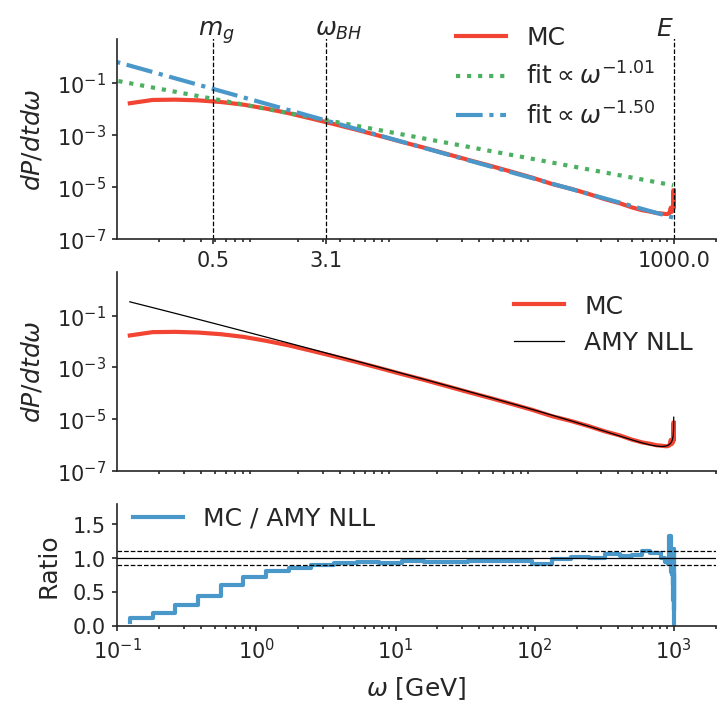
\includegraphics[width=\columnwidth]{spectrum.png}
\caption{The $q\rightarrow q+g$ splitting rate in an infinite medium from a quark with $E=1$ TeV,and a coupling constant $\alpha_s = 0.1$. The top plot shows the simulated spectrum $dR/d\omega$ (red-dashed line) and power law fit (green-dotted and blue-dash-dotted lines) in different gluon energy regions, separated by energy scales $\omega_{BH}\approx 2\pi T$. The middle plot compares to the simulation to NLL solution to the AMY equation, and the ratio is shown in the bottom plot}
\label{fig:spectrum}
\end{figure}

\begin{figure}
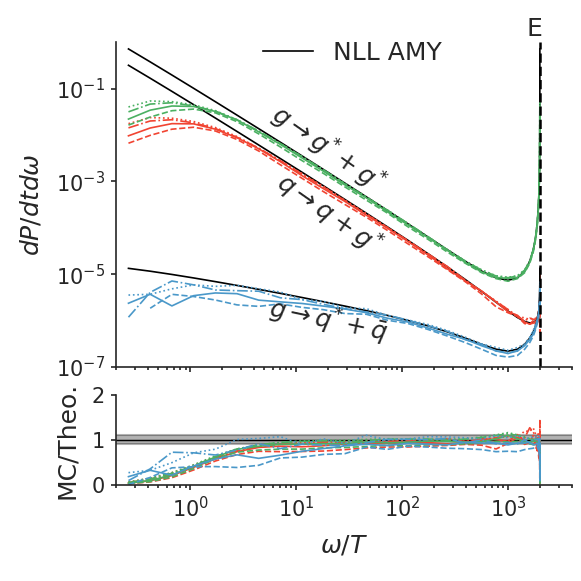
\includegraphics[width=\columnwidth]{channel_rate.png}
\caption{The splitting rate of $q\rightarrow q+g^*$, $g\rightarrow g+g^*$, and $g\rightarrow q^* + \bar{q}$ as a function of the parton energy labeled by the star. The mother parton with $E=1$ TeV evolves inside an infinite medium with $T=0.5$ GeV. The simulations (thick dashed lines) are compared to the NLL solutions (thin solid lines).}
\label{fig:channel_rate}
\end{figure}

\begin{figure}
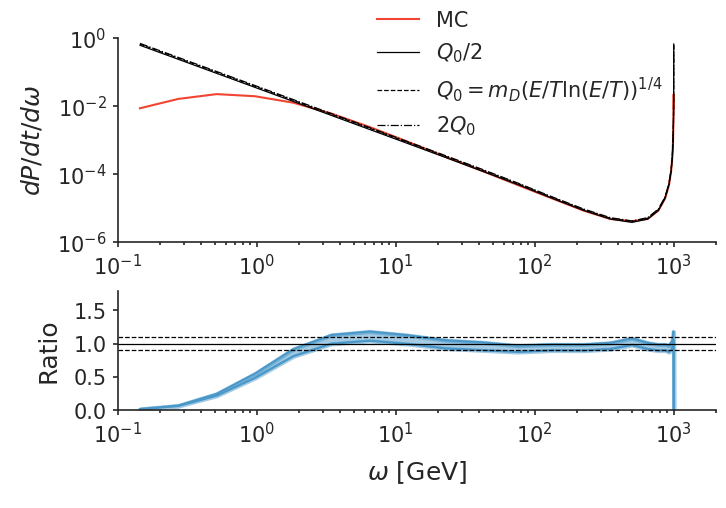
\includegraphics[width=\columnwidth]{running.png}
\caption{Top plot: comparison of modified Boltzmann simulation with the NLL solution  with running coupling.
Three initial guesses of the 
The ratio between simulation and theory is shown in the bottom plot.}
\label{fig:running}
\end{figure}

In this section, we compare the splitting rate $dR/d\omega$ that comes out of the modified Boltzmann approach simulation to the NLL approximation in the infinite medium limit.

The differential rate in an infinite medium $dR/d\omega$ is shown in Figure \ref{fig:spectrum} for a 1 TeV quark splitting into a gluon and a quark.
The temperature of the medium is $T=0.5$ GeV, and a rather small coupling constant $\alpha_s = 0.1$.
Please also refer to Appendix \ref{app:tune-spectrum} for a full comparison varying both the parton energy and the coupling constant.
The horizontal axis is the radiated gluon energy.
In the upper plot, we divided the spectrum into different regions by the gluon thermal mass $m_\infty$ and an estimated Bethe-Heitler energy $\lambda_g m_D^2 \sim 2\pi T$.
The spectrum with above the is suppressed due the use of a finite mass.
In the Bethe-Heitler region $\omega < 2\pi T$, the spectrum scales like $\omega^{-1}$ which comes from the incoherent radiation rate.
In the LPM region $2\pi T < \omega < E$, the spectrum is dominated by coherent multiple scatterings and scales like $\omega^{-3/2}$.
The power-law fits in each domain are very close to the expected scaling.
In the middle plot, we compare the simulation to the NLL solution with self-consistent $Q_1^2$ from Eq. \ref{eq:Q1-sf}. 
The ratio between the two is shown in the bottom plot.
There is a good agreement in the LPM region between the simulation and the theory calculation, which we have used as guidance in developing our Monte-Carlo approach.

A comparison of the other channels $g\rightarrow g+g$ and $g\rightarrow q+\bar{q}$ to the theory calculations are shown in Figure \ref{fig:channel_rate}.
For the splitting parton energy much greater than temperature $\omega > 10 T$, the simulation agrees well with the theory. 

Finally, we compare the running coupling calculation with the theory curve in Fig. \ref{fig:running} for the $g\rightarrow g+g$ channel.
The theory curves (black lines) are obtained combining Eq. \ref{eq:AMY-LL} and Eq. \ref{eq:q3running}.
Different line styles correspond to the variation of the $Q_0$ value around an initial guess $m_D (E/T \ln(E/T) )^{1/4}$ by a factor of $2$ above and below.
For this 1 TeV parton, the scale $Q_0$ is actually very large and the running of $\alpha_s$ is rather slow, which explains the theory curve is not very sensitive to a factor of $4$ change in $Q_0$.
The simulation was performed using the running coupling prescription described in Section \ref{section:running}.
The overall shape of the spectrum in the deep LPM region is again well described by the modified Boltzmann simulation. 


In the previous section, we have shown that the modified Boltzmann equation simulation has a good agreement with the theoretical calculation for parton splitting in the LPM regime in an infinite medium.
Towards future phenomenological application, we would like to investigate a few more complex scenarios involving finite and expanding medium.

For calculation in a finite medium, there is an intricate interference pattern near the boundary which requires solving the original equation using a finite medium temperature profile. 
Or for the case of a thin medium, such effect can be analyzed order by order in the ``opacity ($L/\lambda$) expansion". 
One important effect in a finite medium is the path-length dependent radiation rate for $L \lesssim \tau_f$, which is important for heavy-ion collisions phenomenology, considering the formation time of very energetic splitting can be comparable to the size of the QGP fireball.
Though the modified Boltzmann approach has been constructed to mimic the rate $dR/d\omega$ in the infinite medium limit, and does not recover the exact form of spectrum for a finite medium, it still predicts an $L$-dependent rate and we would like to check whether it is significantly different from the theory expectation.
The origination of the path-length dependence in the modified Boltzmann approach is that the gluons sampled at $t=t_0$ are not considered as independent objects until $t = t_0+\tau_f$, meaning the splittings at time $t$ is initiated by inelastic processes at $t-\tau_f$.
As a result, in a semi-infinite medium with a step function like temperature profile, 
\begin{eqnarray}
T = \begin{cases}
0 , z<0\\
T_0, z>0
\end{cases}
\end{eqnarray}
there are no scattering centers at $L-\tau_f<0$ and thus introduces a reduction in the radiation rate for small path-length.

\begin{figure}
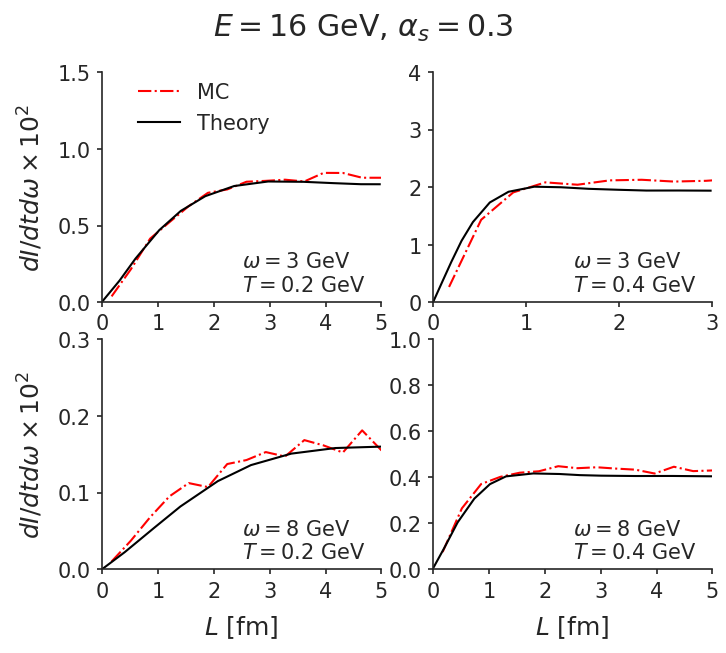
\includegraphics[width=\columnwidth]{spectrum_L.png}
\caption{Comparison of the path-length dependent rate $dR/d\omega$ from the simulation using $\alpha_s = 0.3$ to the theoretical calculation for splitting $q\rightarrow q+g$ \cite{CaronHuot:2010bp}. The quark energy is $16$ GeV.}
\label{fig:spectra-L-alphas=0.3}
\end{figure}

In Figure \ref{fig:spectra-L-alphas=0.3}, the $q\rightarrow q+g$ rate simulated in a semi-infinite medium is compared to the full calculations obtained in \cite{CaronHuot:2010bp}.
The energy of the quark is 16 GeV, and $\alpha_s = 0.3$.
The medium temperature of the left and the right columns are 0.2 GeV and 0.4 GeV respectively.
Top and bottom rows show the differential rates for the emitted gluon  energy $\omega = 3$ GeV and $\omega = 8$ GeV \footnote{In practical simulation, the rate are obtained by counting gluons within a finite energy range $\omega\pm 0.5$ GeV}.
The different rate $dR/d\omega$ are plotted as function of the path length $L$.
It is evident that theoretical rates (black solid lines) first grow approximately linearly with $L$ and then bend over to transit to $L$-independent ones.
The simulation describes the large $L$ limit well and also approximately captures the point at which the transition happens.
But there are systematic deviations compared to the theory at small path-length.
Therefore it will be of great interest to improve to the current simulation approach at small path-length in the future. 
For example, one possible solution would be using the results from the opacity expansion in the simulation for those splittings that happened close to the boundary and developing matching conditions to the approach we used for the deep LPM regime.

\begin{figure}
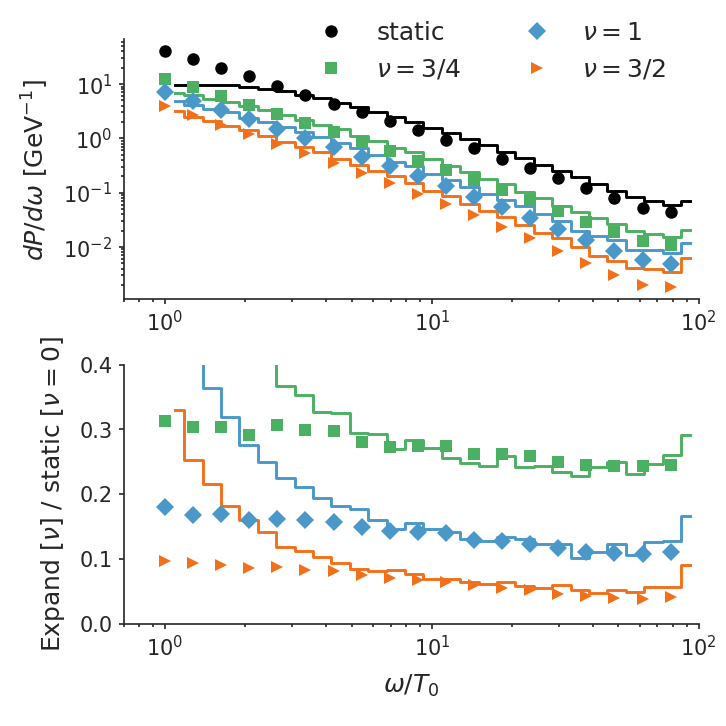
\includegraphics[width=\columnwidth]{spectrum_Bjorken.png}
\caption{The ratios of induced splitting rate in expanding medium to that of a stat medium, with expansion parameter $\nu = 3/4, 1$, and $3/2$. The analytic results are shown in solid lines and simulations denoted as symbols. The conpling constant $\alpha_s=0.3$, the expansion starts at $\tau_0 = 0.2$ fm/$c$ with an initial temperature $T_0 = 1$ GeV.}
\label{fig:Bjorken-BDMPS}
\end{figure}

The expansion of the medium is another important aspects for heavy-ion collision phenomenology.
The created QGP fireballs undergo dramatic expansion, causing the medium temperature at mid-rapidity to drop quickly in the first few fm$/c$.
This introduces another macroscopic scale in additional to the path length, which is the inverse medium expansion rate. 
In the context of this work, we shall define this expansion time scale as the inverse changing rate of $T^3$,
\begin{eqnarray}
\tau_{\textrm{ex}} = \left(\frac{d\ln(T^3)}{d \tau} \right)^{-1},
\end{eqnarray}
to be understood as the time scale over which the local $\hat{q}\propto T^3$ changes notably.
For simplicity, parametrize the temperature profile as a power law fall-off function of the proper time at mid-rapidity,
\begin{eqnarray}
T(\tau; \nu)^3 = T_0^3\left(\frac{\tau_0}{\tau}\right)^{2-1/\nu},
\end{eqnarray}
where the static case is recovered when $\nu=1/2$, and $\nu=1$ corresponds to the temperature profile of a Bjorken flow.
The resultant expansion time scale is
\begin{eqnarray}
\tau_{\textrm{ex}} = \frac{\tau}{2-1/\nu}.
\end{eqnarray}
If this time scale is smaller than the formation time of the splitting, then the medium cannot be well approximated by having a constant temperature when we resumes the multiple scatterings.
Fortunately, in the current modified Boltzmann approach, since we propagate the splitting process in real time, the fast changing of the medium temperature does affect the multiple scatterings that contribute to this specific splitting.

We would like to compare the response of the modified Boltzmann approach to an expanding medium to theoretical calculations.
The theoretical formula we used is obtained in the BDMPS framework 
by the authors of \cite{Baier:1998yf} using the power law type temperature profile. 
The total splitting probability is,
\begin{eqnarray}
\frac{dP}{d\omega} &=& \frac{\alpha_s}{2\pi E}P_{q\rightarrow qg}(x)\mathfrak{Re}\int_{\tau_0}^{\tau_0+L}\frac{dt_f}{t_f}\int_{\tau_0}^{t_f}\frac{dt_i}{t_i} \frac{1}{\nu^2}\\
\nonumber
&& \left.\left[ I_{\nu-1}(z_i)K_{\nu-1}(z_f)-I_{\nu-1}(z_f)K_{\nu-1}(z_i)\right]^{-2}\right|_{\omega}^{\omega=\infty},\\
z_{i,f} &=& 2i\nu \sqrt{\frac{\hat{q}_g(1-x+C_F/C_A x^2)}{2(1-x)\omega}} \tau_0 \left( \frac{t_{i,f}}{\tau_0}\right) ^{1/2\nu}
\end{eqnarray}
for the $q\rightarrow q+g$ splitting.
For $\nu=1/2$, this expression reduces to the static BDMPS result \cite{Baier:1996kr}. 

As a remark, the BDMPS calculation considers the multiple-soft limit of the collision kernel and therefore does not include the logarithm that comes from the perturbative tail $1/q_\perp^4$. 
Accordingly, we turn off the large-$Q$ matrix-element scatterings and only retain diffusion plus diffusion-induced radiation components in our simulation.
Besides, $b=0.75$ is used without the logarithmic correction factor in Eq. \ref{eq:NLL-b}, and the same $\hat{q}_g = m_D^2 C_A\alpha_s T$ are input to the theory and the simulation.
To suppress other difference in the simulation and the theory, instead of making direct comparison of the spectrum $dP/d\omega$ to the BDMPS result, we compare the ratio of the splitting probability in an expanding medium to that of a static medium
\begin{eqnarray}
R_\nu = \frac{dP(T=T(\tau;\nu))/d\omega}{dP(T=T_0)/d\omega}
\end{eqnarray}
between simulation and theory to focus on the response to a fast dropping temperature profile compared to the static case.

The medium expansion starts at $\tau_0=0.2$ fm/$c$ with $T_0=1$ GeV and stops at $\tau = 20$ fm/$c$.
We take four choices of the expansion rate $\nu = 1/2, 3/4, 1, 3/2$, corresponding to a static medium, a slowly expanding medium, Bjorken flow, and a faster-than-Bjorken expansion respectively.
The ratio $R_\nu$ from both theory and simulation are shown in Fig. \ref{fig:Bjorken-BDMPS} for a 100 GeV quark with $\alpha_s=0.3$.
Again, for $\omega/T \gg 1$, the simulation displays the expected decreasing of medium-induced radiation due to the dropping of temperature.
In the future, we are looking forward to making direct comparison to the solution of Eq. \ref{eq:full-theory} with both varying temperature and adding medium flow effects.

\subsection{Summary}
We have investigated the modification to the incoherent Boltzmann transport approach to include the LPM effect for parton splitting processes in the deep LPM region, with the guidance from the LL and the NLL solutions of the AMY equation.
The running coupling effect has also been implemented in this approach.
The overall level of agreement between the simulated results and theoretical calculations in the infinite medium limit is promising given the simplicity and limits of this Monte-Carlo procedure. 
Although it was developed for the deep LPM regime, the current approach captures qualitative features of the path-length dependence of medium induced splittings and the qualitative change of the spectrum shape in an expanding medium compared to the static case.
Of course, it is important to improve this method for the case of a thin medium.
Another interest of study would be a consistent inclusion of the heavy quark mass effect into the current approach.
We shall seek for improvements in these aspects in future works.

Designing such a modified Boltzmann transport approach and performing systematic comparison to theoretical calculations have allowed us to reduce and estimate the uncertainty in implementing the medium-induced splitting processes in the transport models. 
This is instrumental for performing an examination of theory assumptions and a more meaningful phenomenological extraction of jet transport properties from future model-to-data comparison in transport model based studies.

\begin{figure}
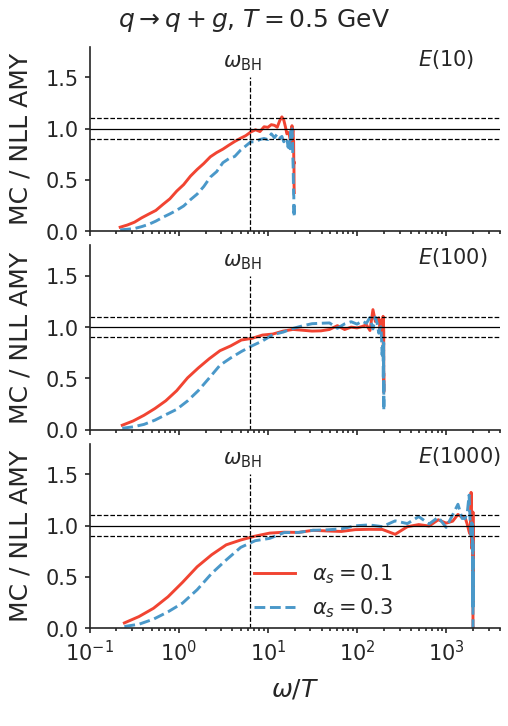
\includegraphics[width=.5\columnwidth]{spectrum_E_q2qg.png}
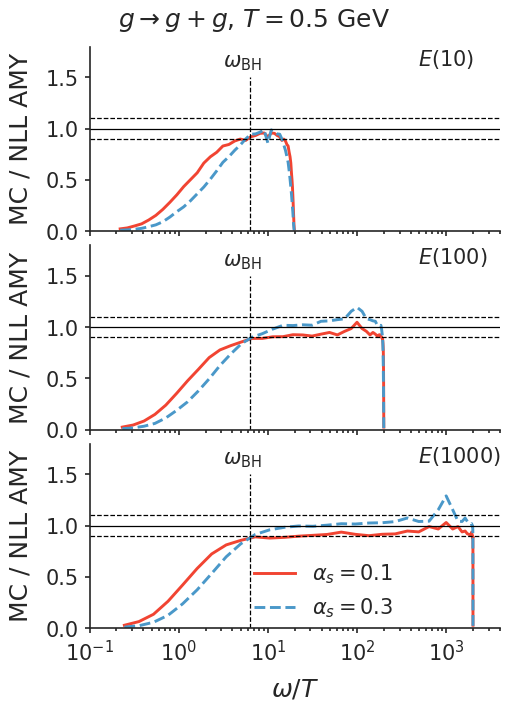
\includegraphics[width=.5\columnwidth]{spectrum_E_g2gg.png}
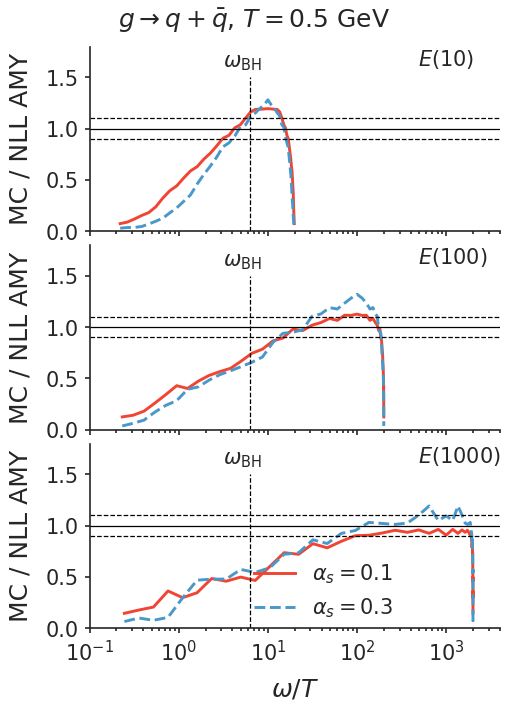
\includegraphics[width=.5\columnwidth]{spectrum_E_g2qqbar.png}
\caption{Ratios of splitting rate $dR/\omega$ between the modified Boltzmann simulation and the NLL solution for $q\rightarrow q+g$ splitting. The quark energies are $E$ is 10, 100, and 100 GeV from top to the bottom plot. 
And two coupling constants are used: $\alpha_s = 0.1$ (red solid lines) and $\alpha_s = 0.3$ (blue dashed lines).
$\omega$ stands for the gluon energy.
The horizontal dashed lines denote $\pm 10\%$ deviation from unity. }
\label{fig:q2qg}
\end{figure}

In this appendix, we provide comparisons of splitting rate at different values of energy and coupling constant for the reader's references.
Fig. \ref{fig:q2qg}, Fig. \ref{fig:g2gg} and Fig. \ref{fig:g2qqbar} shows the comparison for channels $q\rightarrow q+g$, $g\rightarrow g+g$ and $g\rightarrow q+\bar{q}$ respectively.
The results are shown as the ratio between the simulations and the NLL solution.
Within in each figure, the mother parton energy are 10 GeV, 100 GeV and 1000 GeV from the top to bottom plot.
We have used two coupling constants at $\alpha_s = 0.1$ (red solid lines) and $\alpha_s = 0.3$ (blue dashed lines).

\subsection{Hard matrix-elements}

The vacuum matrix-elements are,
\begin{eqnarray}
\overline{|M_{22,Qq}|^2} &=& \frac{64\pi^2\alpha_s^2}{9} \frac{(M^2-u)^2 + (s-M^2)^2 + 2 M^2 t}{t^2}
\nonumber
\\
\overline{|M_{22,Qg}|^2} &=& \pi^2 \left\{
32\alpha_s^2 \frac{(s-M^2)(M^2-u)}{t^2} \right.
\nonumber
\\
&+&\frac{64}{9}\alpha_s^2 \frac{(s-M^2)(M^2-u)+2M^2(s+M^2)}{(s-M^2)^2} \nonumber
\\
&+&\frac{64}{9}\alpha_s^2 \frac{(s-M^2)(M^2-u)+2M^2(u+M^2)}{(M^2-u)^2} \nonumber
\\
&+& \frac{16}{9}\alpha_s^2 \frac{M^2(4M^2 - t)}{(M^2-u)(s-M^2)} 
\nonumber
\\
&+& 16 \alpha_s^2 \frac{(s-M^2)(M^2-u)+M^2(s-u)}{t(s-M^2)}
\nonumber
\\
&-& \left. 16 \alpha_s^2 \frac{(s-M^2)(M^2-u)-M^2(s-u)}{t(M^2-u)}\right\}
\nonumber
\\
|M_{2\rightarrow 3}|^2 &=& |M_{2\rightarrow 2}|^2 48 \pi \alpha_s (1-\bar{x})^2
\nonumber
\\
&\times&\left(\frac{\vec{k}_\perp}{k_\perp^2 + x^2 M^2} + \frac{\vec{q}_\perp - \vec{k}_\perp}{(\vec{q}_\perp-\vec{k}_\perp)^2 + x^2 M^2}
\right)^2 
\end{eqnarray}
In medium, the denominator of the squared gluon propagator is replaced by $t^2 \rightarrow t(t-m_D^2)$. 
For the radiation processes, we also include a gluon mass to regulate soft divergence $x^2M^2 \rightarrow x^2M^2 + (1-x)m_g^2$, where $m_g^2 = m_D^2/2$ is the squared asymptotic gluon mass. 

\begin{figure}
\centering
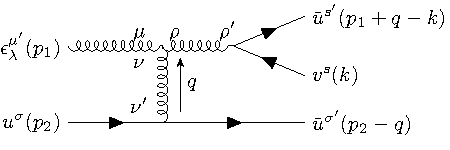
\includegraphics[width=.5\textwidth]{Large-Q-g2qqbar-A.pdf}\\
\vspace{1em}
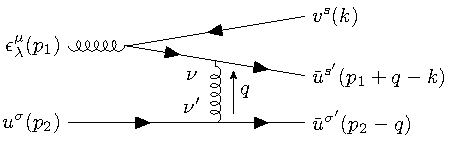
\includegraphics[width=.49\textwidth]{Large-Q-g2qqbar-B.pdf}\hfill
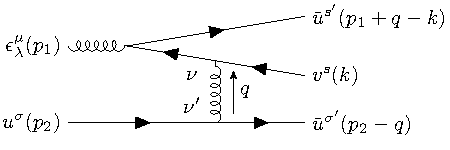
\includegraphics[width=.49\textwidth]{Large-Q-g2qqbar-C.pdf}
\caption{Three diagrams $A$ (Top), $B$ (Bottom left), $C$ (Bottom right) that contribute to the large angle scattering induced gluon splitting into quark-anti-quark pair.}
\end{figure}


\begin{eqnarray}
p_1 &=& (\sqrt{s}, 0, \vec{0})\\
p_2 &=& (0, \sqrt{s}, \vec{0})\\
k &=& (x\sqrt{s}, \frac{k_\perp^2}{x\sqrt{s}}, \vec{k}_\perp)\\
q &\sim& (-\frac{q_\perp^2}{\sqrt{s}}, \frac{q_\perp^2 + k_\perp^2/x - 2\vec{q}_\perp \cdot \vec{k}_\perp}{(1-x)\sqrt{s}}, \vec{k}_\perp)\\
n &=& (0, 1, 0)\\
\epsilon(p) &\sim& (0, \frac{2\vec{\epsilon}_\perp\cdot\vec{p}_\perp}{p^+}, \vec{\epsilon}_\perp)
\end{eqnarray}

The first diagram:
\begin{eqnarray}
i M_A &=& (-ig)^2(-g)f^{abc}(t^b)_{j'j}(t^c)_{i'i} \epsilon_\lambda^\mu(p_1) \\\nonumber
&&\frac{-i}{(p_1+q)^2}\left(g^{\rho\rho'}-\frac{n^{\rho}(p_1+q)^{\rho'}+n^{\rho'}(p_1+q)^\rho}{n\cdot (p_1+q)}\right) \bar{u}^s(p_1+q-k)\gamma_{\rho'}v^{s'}(k) \\ \nonumber
&&\frac{-i}{q^2}\left(g^{\nu\nu'}-\frac{n^{\nu}q^{\nu'}+n^{\nu'}q^\nu}{n\cdot q}\right) \bar{u}^{\sigma}(p_4)\gamma_{\nu'}u^{\sigma'}(p_2) \\ \nonumber
&& \left[g_{\mu\nu}(p_1-q)_\rho + g_{\nu\rho}(2q+p_1)_\rho + g_{\rho\mu}(-2p_1 -q)_\nu \right]\\
&\approx& -g^3 f^{abc}(t^b)_{j'j}(t^c)_{i'i} \delta^{\sigma\sigma'} \epsilon^\mu(p_1) \\\nonumber
&&\frac{1}{(p_1+q)^2} \sum_{\lambda'=\pm}\epsilon_{\lambda'}^{\rho}(p_1+q)\underbrace{\epsilon_{\lambda'}^{*,\rho'}(p_1+q) \bar{u}^s(p_1+q-k)\gamma_{\rho'}v^{s'}(k)}_{iP_{A,\lambda'}^{ss'}} \\ \nonumber
&&\frac{1}{q_\perp^2}\left(g^{\nu\nu'}-\frac{n^{\nu}q^{\nu'}+n^{\nu'}q^\nu}{n\cdot q}\right) (2p_2-q)_{\nu'} \\ \nonumber
&& \left[g_{\mu\nu}(p_1-q)_\rho + g_{\nu\rho}(2q+p_1)_\rho + g_{\rho\mu}(-2p_1 -q)_\nu \right] \\
&=& -g^3 f^{abc}(t^b)_{j'j}(t^c)_{i'i} \frac{1}{(p_1+q)^2}\frac{1}{q_\perp^2} \sum_{\lambda'=\pm}iP_{A,\lambda}^{ss'} \delta^{\sigma\sigma'}  \\ \nonumber
&& \epsilon_\lambda^\mu(p_1)2p_2^{\nu} \epsilon_{\lambda'}^{\rho}(p_1+q) \left[g_{\mu\nu}(p_1-q)_\rho + g_{\nu\rho}(2q+p_1)_\rho + g_{\rho\mu}(-2p_1 -q)_\nu \right]\\
&\approx& -g^3 f^{abc}(t^b)_{j'j}(t^c)_{i'i}\delta^{\sigma\sigma'}\frac{2s}{q_\perp^2} \frac{x(1-x)}{(\vec{k}_\perp-x \vec{q}_\perp)^2} iP_{A,\lambda}^{ss'} 
\end{eqnarray}
The second and third diagram,
\begin{eqnarray}
i M_B &=& i g^3 (t^b t^a)){i'i} t^b{j'j} \delta^{\sigma\sigma'} \frac{2s}{q_\perp^2} \frac{x(1-x)}{k_\perp^2}  iP_{B,\lambda}^{ss'} \\
i M_C &=& -i g^3 (t^a t^b)){i'i} t^b{j'j} \delta^{\sigma\sigma'} \frac{2s}{q_\perp^2} \frac{x(1-x)}{(\vec{k}_\perp-\vec{q}_\perp)^2}  iP_{C,\lambda}^{ss'} 
\end{eqnarray}
The sum of all three diagrams, applying $f^{abc}t^c = -i[t^a, t^b]$
\begin{eqnarray}
i (M_A+M_B+M_C) &=& ig^3 \frac{2s}{q_\perp^2} (t^b)_{j'j} x(1-x)\\\nonumber
&&\left\{(t^a t^b)_{i'i} \left(\frac{iP_{A,\lambda}^{ss'} }{(\vec{k}_\perp-x \vec{q}_\perp)^2} - \frac{iP_{C,\lambda}^{ss'}}{(\vec{k}_\perp-\vec{q}_\perp)^2}\right) -(t^a t^b)_{i'i}\left(\frac{iP_{A,\lambda}^{ss'} }{(\vec{k}_\perp-x \vec{q}_\perp)^2} - \frac{iP_{B,\lambda}^{ss'}}{k_\perp^2}\right) \right\}
\end{eqnarray}


The splitting amplitude:
\begin{eqnarray}
&&\epsilon_{\lambda, \mu} \bar{u}_s(a)\gamma^\mu v_{s'}(b)\\
&=&\frac{1}{\sqrt{2a}\sqrt{2b}}(\xi^T_s a\cdot\sigma, \xi^T_{s} a\cdot \bar{\sigma})
\begin{bmatrix}
\epsilon\cdot\bar{\sigma} & 0 \\
0 & \epsilon\cdot\sigma
\end{bmatrix}
\begin{bmatrix}
b\cdot\sigma \eta_{s'}\\
b\cdot\bar{\sigma} \eta_{s'}
\end{bmatrix}
\\
&=&\frac{1}{2\sqrt{ab}}
\xi_s^T
\begin{bmatrix}
a^- & -a^\perp_L \\
-a^\perp_R & a^+
\end{bmatrix}
\begin{bmatrix}
0 & \sqrt{2}\delta_{\lambda R}\\
\sqrt{2}\delta_{\lambda L} & \frac{\sqrt{2}c^\perp_\lambda}{c^+}
\end{bmatrix}
\begin{bmatrix}
b^- & -b^\perp_L \\
-b^\perp_R & b^-
\end{bmatrix}
\eta_{s'}\\\nonumber
&-&
\frac{1}{2\sqrt{ab}}
\xi_s^T
\begin{bmatrix}
a^+ & a^\perp_L \\
a^\perp_R & a^-
\end{bmatrix}
\begin{bmatrix}
\frac{\sqrt{2}c^\perp_\lambda}{c^+} & -\sqrt{2}\delta_{\lambda R}\\
-\sqrt{2}\delta_{\lambda L} & 0
\end{bmatrix}
\begin{bmatrix}
b^+ & b^\perp_L \\
b^\perp_R & b^-
\end{bmatrix}
\eta_{s'}
\\
&=&\frac{1}{\sqrt{2ab}}
\xi_s^T
\begin{bmatrix}
-a^\perp_L b^- \delta_{\lambda L} - a^- b^\perp_L \delta_{\lambda R} + a^\perp_L b^\perp_R\frac{c^\perp_\lambda}{c^+} &
-a^\perp_L b^\perp_L \delta_{\lambda L} + a^- b^+ \delta_{\lambda R} + a^\perp_L b^+\frac{c^\perp_\lambda}{c^+}
\\
a^+ b^- \delta_{\lambda L} + a^\perp_R b^\perp_R \delta_{\lambda R} - a^+ b^\perp_R\frac{c^\perp_\lambda}{c^+} &
-a^+ b^\perp_L \delta_{\lambda L} - a^\perp_R b^+ \delta_{\lambda R} + a^+ b^+\frac{c^\perp_\lambda}{c^+}
\end{bmatrix}
\eta_{s'}\\\nonumber
&-&\frac{1}{\sqrt{2ab}}
\xi_s^T
\begin{bmatrix}
-a^\perp_L b^+ \delta_{\lambda L} - a^+ b^\perp_R \delta_{\lambda R} + a^+ b^+\frac{c^\perp_\lambda}{c^+} &
-a^\perp_L b^\perp_L \delta_{\lambda L} - a^+ b^- \delta_{\lambda R} + a^+ b^\perp_L\frac{c^\perp_\lambda}{c^+}
\\
-a^- b^+ \delta_{\lambda L} - a^\perp_R b^\perp_R \delta_{\lambda R} + a^\perp_+ b^+\frac{c^\perp_\lambda}{c^+} &
-a^- b^\perp_L \delta_{\lambda L} - a^\perp_R b^- \delta_{\lambda R} + a^\perp_R b^\perp_L\frac{c^\perp_\lambda}{c^+}
\end{bmatrix}
\eta_{s'}
\end{eqnarray}
Dropping terms that is of order $(+)(-)$ or $(\perp)(\perp)$ or $(\perp)(-)$,
\begin{eqnarray}
&&\epsilon_{\lambda, \mu} \bar{u}_s(a)\gamma^\mu v_{s'}(b)\\
&=& \frac{1}{\sqrt{2ab}}
\xi_s^T
\begin{bmatrix}
a^\perp_L b^+ \delta_{\lambda L} + a^+ b^\perp_R \delta_{\lambda R} - a^+ b^+\frac{c^\perp_\lambda}{c^+} & 0\\
0 & -a^+ b^\perp_L \delta_{\lambda L} - a^+ b^\perp_R \delta_{\lambda R} + a^+ b^+\frac{c^\perp_\lambda}{c^+}
\end{bmatrix}
\eta_{s'}
\end{eqnarray}
The module square of one splitting amplitude, sum over spins and average over polarization is ($a^+ = xc^+, b^+ = (1-x)c^+$ and $c = a+b$),
\begin{eqnarray}
\frac{1}{2}\sum_\pm |P|^2 = \frac{2(x^2 + (1-x)^2)}{x(1-x)} \left((1-x)\vec{a}_\perp-x\vec{b}_\perp\right)^2.
\end{eqnarray}
This result goes back to the standard splitting function if it is computed in the frame where $a_\perp = -b_\perp$. 
However, there is no such frame that $a_\perp = -b_\perp$ satisfies simultaneously for the splitting in diagram A, B and C, therefore the result gets complicated,
\begin{eqnarray}
\frac{1}{2d_F 2d_A}\sum_{\lambda, s, s', \sigma, \sigma', a, b}|M^2|_{g+q\rightarrow q+\bar{q}+q} &=& g^6 \frac{2C_F}{d_A}\frac{4s^2}{q_\perp^4}x(1-x)\overbrace{\frac{(x^2+(1-x)^2)}{2}}^{P(x)}  \\\nonumber
&\times&\left(C_F \vec{A}^2 + C_F \vec{B}^2 - (2C_F- C_A)\vec{A}\cdot\vec{B}\right)
\end{eqnarray}
Where the $\vec{A}$ and $\vec{B}$ is,
\begin{eqnarray}
\vec{A} &=& \frac{\vec{k}_\perp - x\vec{q}_\perp}{(\vec{k}_\perp - x\vec{q}_\perp)^2} -  \frac{\vec{k}_\perp - \vec{q}_\perp}{(\vec{k}_\perp - \vec{q}_\perp)^2} \\
\vec{B} &=& \frac{\vec{k}_\perp - x\vec{q}_\perp}{(\vec{k}_\perp - x\vec{q}_\perp)^2} -  \frac{\vec{k}_\perp}{\vec{k}_\perp^2}
\end{eqnarray}

Similarly for $g+q\rightarrow g+g+q$, and $q+q\rightarrow q+g+q$
\begin{eqnarray}
\overline{|M^2|}_{g+q\rightarrow g+g+q} &=& g^6 \frac{C_A}{d_F}\frac{4s^2}{q_\perp^4}x(1-x) ]\overbrace{C_A\frac{1+x^4+(1-x)^4}{x(1-x)}}^{P(x)}   \\\nonumber
&\times&\left(\vec{A}^2 + \vec{B}^2 - \vec{A}\cdot\vec{B}\right)\\
\vec{A} &=& \frac{\vec{k}_\perp - x\vec{q}_\perp}{(\vec{k}_\perp - x\vec{q}_\perp)^2} -  \frac{\vec{k}_\perp - \vec{q}_\perp}{(\vec{k}_\perp - \vec{q}_\perp)^2} \\
\vec{B} &=& \frac{\vec{k}_\perp - x\vec{q}_\perp}{(\vec{k}_\perp - x\vec{q}_\perp)^2} -  \frac{\vec{k}_\perp}{\vec{k}_\perp^2}
\end{eqnarray}

and

\begin{eqnarray}
\overline{|M^2|}_{g+q\rightarrow g+g+q} &=& g^6 \frac{C_F}{d_F}\frac{4s^2}{q_\perp^4}x(1-x) \overbrace{C_F\frac{1+(1-x)^2}{x}}^{P(x)}  \\\nonumber
&\times&\left(\vec{A}^2 + \vec{B}^2 - \left(2-\frac{C_A}{C_F}\right)\vec{A}\cdot\vec{B}\right)\\
\vec{A} &=& \frac{\vec{k}_\perp - \vec{q}_\perp}{(\vec{k}_\perp - \vec{q}_\perp)^2} -  \frac{\vec{k}_\perp - x\vec{q}_\perp}{(\vec{k}_\perp - x\vec{q}_\perp)^2} \\
\vec{B} &=& \frac{\vec{k}_\perp - \vec{q}_\perp}{(\vec{k}_\perp - \vec{q}_\perp)^2} -  \frac{\vec{k}_\perp}{\vec{k}_\perp^2}
\end{eqnarray}
